\documentclass[linenumbers,trackchanges,twocolumn]{aastex701}
\usepackage{graphicx}
\usepackage{multirow}
\graphicspath{{figures/}}
\newcommand{\todo}[1]{{$\blacksquare$~\textbf{\color{red}#1}~$\blacksquare$}}

\DeclareRobustCommand{\Eqref}[1]{Eq.~\ref{#1}}
\DeclareRobustCommand{\Figref}[1]{Fig.~\ref{#1}}
\DeclareRobustCommand{\Tabref}[1]{Tab.~\ref{#1}}
\DeclareRobustCommand{\Secref}[1]{Sec.~\ref{#1}}

%%%%%%%%%%%%%%%%%%%%%%%%%%%%%%%%%%%%%%%%%%%%%%%%%%%%%%%%%%%%%%%%%%%%%%%%%%%%%%%%
% If you want to update directly the text, please use a custom color
%
% \newcommand{\yourname}[1]{\textcolor{green!75!black}{#1}}
%
% copy/uncomment the line above, edit the string <yourname> and color (avoid
% red, you can blend colors (the example above is 75% green and 25% black).
% Then in the manuscript do \yourname{your text}.
% Please don't leave overleaf comments as I will not see them.
%%%%%%%%%%%%%%%%%%%%%%%%%%%%%%%%%%%%%%%%%%%%%%%%%%%%%%%%%%%%%%%%%%%%%%%%%%%%%%%%

\begin{document}

\title{A grid of fast-rotating, chemically-homogeneous, supernova and/or long-GRB progenitors}

\author[0000-0002-6718-9472]{M.~Renzo}
\affiliation{Steward Observatory, Department of Astronomy, University of Arizona, 933 N. Cherry Ave., Tucson, AZ 85721, USA}
\email{mrenzo@arizona.edu}

\author[]{\todo{TBD}}
\affiliation{\todo{somewhere}}
\email{\todo{someone@somewhere.edu}}

%% Ore? Leon? Koushik, Aldana, Neev, Matteo, Jared? Carl?

\begin{abstract}
  %
  The understanding of stellar collapse and explosion has rapidly
  matured in recent years, and uncertainties in the progenitor profile
  at the onset of collapse are often dominant.
  %
  We present a grid of 113 stellar models with initial masses
  $M_{\rm ZAMS}=30-90\,M_{\odot}$ and initial rotation
  $\omega_{\rm ZAMS}/\omega_{\rm crit}=0.5-0.99$ computed with
  \textsc{MESA}. We adopt a 128-isotope nuclear reaction network
  capable of self-consistently capture the weak reactions
  deleptonizing the core during and after silicon core burning. By
  construction, these models experience rotationally-induced
  chemically-homogeneous evolution, and reach the onset of collapse
  core-collapse ($v_{\rm infall}\lesssim -300\,\mathrm{km\ s^{-1}}$)
  with sufficient rotation to form accretion disks on the
  proto-compact object.
  %
  Therefore, these progenitor structures provide a homogeneous
  playground with updated input physics and improved algorithmic
  accuracy to understand possibly-jetted stellar explosions, and long
  gamma ray bursts specifically.
\end{abstract}

\keywords{\uat{High Energy astrophysics}{739} --- \uat{Stellar astronomy}{1583} --- }

\section{Introduction}
\label{sec:intro}

Understanding how massive stars' iron cores collapse and, at least in
some cases, the collapse successfully reverts into an explosion is a
long-standing problem of astrophysics since the connection between
massive-star populations and supernovae \citep{baade:34}. In the past
$\sim$century, the increased cadence, wavelength coverage, and depth
of time-domain astronomy has lead to variations on this theme
motivated by all kinds of astronomical transients
\citep[e.g.,][]{cano:17}.

The core structure of a stellar progenitor determines the initial
conditions for expensive multi-dimensional, multi-physics, (and often
multi-million-CPUh) simulations. Specifically, the profile (of
density, entropy, velocity, angular momentum, magnetic fields,
etc.,~as a function of Lagrangian mass coordinate or radius)
determines the dynamics of the infalling gas, and the ``over-burden''
encountered by a putative nascent outflow. Therefore, ultimately, it
is the structure of the progenitor that determines whether a stellar
model explodes or not, separately, whether it leaves behind a neutron
star (NS) or a black hole (BH), and the properties of both the
outflows, associated transients, and remnant \citep[e.g.,][]{janka:12,
  burrows:24, gottlieb:25}.

Recent progress in core-collapse supernova (SN) theory has produce
unprecedented agreement among groups performing numerical simulations
of neutrino-radiative transfer \citep[e.g.,][]{janka:12, ott:18, vartanyan:19,
  burrows:25, nakamura:25}. While the impact of ingredients other than
neutrino heating remains debated \cite[e.g.,][]{soker:24}, a consensus
on the fact that uncertainties in the stellar progenitor structure are
dominant is emerging \citep[e.g.,][]{sukhbold:16, limongi:18,
  boccioli:24, burrows:25, griffiths:26}.

The capability to study the origin of transients and compact objects
is ever more important in the era of large time-domain surveys (e.g.,
Rubin/LSST, \citealt{ivezic:19}) and routine detections of
gravitational-wave mergers \citep[e.g.,][]{abac:25, GWTC-5}. The current
bottleneck in these studies is the availability of models of stellar
progenitors computed \emph{i} sufficiently late into the collapse and
\emph{ii} including sufficient physics to capture the known critical
ingredients for the explosion.

Specifically, point \emph{i} requires pushing the stellar evolution
models well into the sub-sonic phase of the collapse, at least beyond
when timescales associated to stellar processes are longer than the
remaining time to core-bounce. This typically means evolving beyond
iron-core infall velocity
$v_{\rm infall} = \min(v) \lesssim -300\,\mathrm{km\ s^{-1}}$
\citep[e.g.,][]{farmer:23, gottlieb:24} if not
$-1000\,\mathrm{km\ s^{-1}}$ \citep[e.g.,][]{woosley:02}. Beyond this
point, matter typically becomes partially optically thick to
neutrinos, and the thermodynamics exceeds the bounds of tabulated
equations of state in stellar evolution codes.

For point \emph{ii}, a stellar model to be used to understand the
explosion physics needs to be as accurate as possible in its density
and angular momentum profile. Any star evolving through silicon core
burning will experience copious amounts of electron captures
\cite[e.g.,][]{arnett:77,hix:93,hix:99,grichener:25} which
progressively de-leptonize the core (i.e., decrease the amount of free
electrons). These occur at a significant rate even in the late
hydrostatic stellar evolution, and before a model is sufficiently
evolved by the criterion \emph{i}. The notable exceptions to this are
``electron-capture'' SN progenitors which collapse with a ONeMg-rich
core (however, these too require appropriate treatment of the weak
reactions, including URCA processes, \citealt{nomoto:84,
  takahashi:13}) and progenitors above the pair-instability gap
\citep[e.g.,][]{rakavy:67, woosley:17, renzo:24} which collapse
because of the photodisintegration instability in an oxygen-rich core
\citep[e.g.,][]{bond:84, gottlieb:25}.

To decrease the computing time and number of models stopped by
numerical issues in a grid of stellar progenitors, a commonly adopted
shortcut is to use small ($\sim$20-isotope) nuclear reaction networks
\citep[e.g.,][]{pols:95, timmes:00}. These bypass the complex nuclear
physics of silicon core burning by lumping all weak interactions in a
custom compound reaction (see \citealt{grichener:25}), effectively
sacrificing the accuracy of the core structure that decides the
explosion. Even if such compound reaction is tuned on the central
value of the electron fraction $Y_{e}$ from models with more accurate
nuclear reaction networks \citep[e.g.,][]{aguilera-dena:18,
  schneider:21, schneider:24}, small networks cannot predict the
\emph{profile} $Y_{e}(m)$ of the collapsing core in the region where
the explosions are decided. While this is an acceptable trade-off to
study, for example, electromagnetic observables determined at the
surface \citep[e.g.,][]{morozova:15}, it is not sufficient if one want
to investigate the driving of the explosions, the pre-explosions and
explosive neutrino signals, the nuclear yields, and the resulting
compact object properties (whether considering non-rotating --
\citealt{farmer:16} -- or rotating progenitors -- \citealt{renzo:24}). The
reason is that the effective Chandrasekhar mass of the collapsing core
scales with $\propto Y_{e}^{2}$, or in other words, the contribution
of electron-degeneracy-pressure to the support of the core amplifies
small imprecision in the core structure to a level significant for the
collapse and explosion dynamics.

Few grids of stellar progenitors evolved sufficiently late (\emph{i})
and with \emph{detailed} nuclear physics (\emph{ii}) exist, mostly
from closed-source codes (e.g., \textsc{KEPLER}
\citealt{weaver:78, woosley:02, woosley:06, woosley:07, sukhbold:16,
  sukhbold:18}, \textsc{FRANEC}\footnote{ which does not include
  hydrodynamics and thus cannot reach condition \emph{i}
  \citep[e.g.,][]{oconnor:10,limongi:20}.} \citealt{limongi:03,
  limongi:18}, \textsc{HOSHI}, \citealt{takahashi:13}). While these
stellar models have been invaluable in allowing the progress made so
far, they do not allow to explore the sensitivity of the results to
\emph{physical} and \emph{numerical} choices in the evolution of the
progenitors, that have been shown to influence the core structure and
thus explosion outcomes \citep[e.g.,][]{farmer:16, renzo:17,davis:19,
  laplace:21, maltsev:25, myers:26}.

A few public grids of progenitors fulfilling both conditions \emph{i}
and \emph{ii} computed with the open-source and community-driven code
\textsc{MESA} exist \citep[e.g.,][]{farmer:16, renzo:17, laplace:21,
  farag:20, farmer:23, myers:26}. These have largely been under-utilized
for initializing explosion simulations \citep[see
however][]{vartanyan:21}. Even fewer open-source models of rotating
progenitors exist, despite their importance for jetted explosions,
collapsars, MHD-explosions, and/or long $\gamma$-ray burst (lGRB,
\citealt{woosley:93,macfadyen:94,gottlieb:25b}).

The reason for this bottleneck is the significant computational cost
of evolved massive stars with the necessary large nuclear-reaction
networks (neglecting the sparsity, the size of the matrix to solve
scales with $\sim{}N^{2}$ with $N$ number of isotopes),
coupled with the stiffness of the equations (see
\citealt{grichener:25}), which results in large fractions of
progenitor grids failing before reaching the desired infall velocity.

Development of numerical strategies to address these issues are
ongoing. In the meantime, we present here a publicly-available grid of
fast-rotating models fulfilling both criteria (\emph{i}, ``late
enough'') and (\emph{ii}, ``including enough nuclear physics to
accurately simulate the structure'') for studies of the collapse and
possible explosion of fast rotating stellar cores.

In \Secref{sec:methods} we describe the physical assumptions and
numerical setup. \Secref{sec:results} presents the computed grid, and
we contextualize our result in terms of the input and code physics in
\Secref{sec:discussion_inputs}. In \Secref{sec:scenario} we briefly
outline the astrophysical scenarios that could be approximated with
our models. Finally, we conclude in
\Secref{sec:conclusion}. Appendix~\ref{sec:table} lists some key quantities for the ``explodability'' and surface composition at the onset of collapse, and Appendix~\ref{sec:public_datafiles} describes
in detail the publicly available input and output files of our
simulations, available at
\href{https://doi.org/10.5281/zenodo.14286306}{doi.org/10.5281/zenodo.14286306}.


\section{Numerical setup}
\label{sec:methods}

The grid of models presented here is an extension of (and includes)
the progenitor star used in \cite{gottlieb:24} and constitutes the
input for the ``averaged'' progenitor constructed in \cite{chan:26}.
We use the \textsc{MESA} code (version r24.03.1,
\citealt{paxton:11,paxton:13,paxton:15,paxton:16,paxton:19,jermyn:23}),
to compute low-metallicity ($Z=0.001$) and fast-rotating stellar
models. Our grid spans initial masses $M_{\rm ZAMS}=30-90\,M_{\odot}$
and initial (rigid) rotation with angular frequency
$\omega_{\rm ZAMS}/\omega_{\rm crit}=0.5-0.99$, where
$\omega_\mathrm{crit}=\sqrt{(1-L/L_\mathrm{Edd})GM/R^3}$ is the
surface critical rotation rate accounting for radiative forces, $L$ is
the stellar luminosity, $L_\mathrm{Edd}$ the Eddington luminosity, $G$
is the gravitational constant, $M$ is the total mass and $R$ the
stellar radius.

We use the \textsc{Skye} equation of state \citep{jermyn:skye}, and
include electron screening following \citet{Chugunov2007} and thermal
neutrino losses following \citet{Itoh1996}. In our setup, radiative
opacities are primarily from OPAL \citep{Iglesias1993, Iglesias1996}
and electron conduction opacities are from \citet{Cassisi2007}.

We adopt nuclear reaction rates that are a combination of NACRE
\citep{Angulo1999}, JINA REACLIB \citep{Cyburt2010}, and
$^{12}\mathrm{C}(\alpha,\gamma)^{16}\mathrm{O}$ from \cite{kunz:02},
plus additional tabulated weak reaction rates \citet{Fuller1985,
  Oda1994, Langanke2000}. To capture with sufficient accuracy the
deleptonization of the core from the structural point of view
(condition \emph{ii} in \Secref{sec:intro}), we adopt the
fully-coupled 128-isotope nuclear reaction network
\texttt{mesa\_128.net} \citep{farmer:16, grichener:25}. For central
temperatures above $\log_{10}(T)\ge 9.2$, we employ \textsc{MESA} in
operator split mode \citep{jermyn:23}.


Throughout the evolution, we include the wind mass loss rate following
\cite{vink:00} and \cite{nugis:00} for surface $^{4}\mathrm{He}$ mass fraction $Y_{\rm surf}\ge0.4$,  assuming the metallicity scaling
from \cite{vink:01} and the rotational enhancement from
\cite{friend:86} \citep[see also][]{langer:98}.

We use the Schwarzschild criterion and the \cite{henyey:65}
formulation of mixing-length theory for convective layers, with
$\alpha_{\rm MLT}=1.5$. For convective boundary mixing, we include
core overshooting as a step-function following \cite{brott:11}
($\alpha_{\rm ov}=0.335$) and treat rotational mixing in diffusion
approximation following \cite{heger:00}, including angular momentum
transport by convection or by a ``classical'' Tayler-Spruit dynamo
\citep{spruit:02} in radiative regions. All the models presented here
result by construction in a rotationally-driven chemically homogeneous
evolution \cite[CHE, e.g.,][]{maeder:00, yoon:06}.

After the formation of a carbon-oxygen core, we prevent the
development of spurious numerical velocities in the outer layers by
artificially setting to zero the velocity in any layer that has a
sound-propagation time from the outer edge of the core, or the
location where the specific entropy drops below 10.5\,$N_{A}k_{B}$,
whichever is further in, longer than the current timestep. Similar
artificial damping exists in most calculations of post-core-carbon
burning massive stars \citep[e.g.,][]{aguilera-dena:18}.

To produce progenitors sufficiently close to core-bounce (condition
\emph{i} in \Secref{sec:intro}), we evolve each model until the infall
velocity in the iron core decreases below
$v_{\rm infall}\le-300\,\mathrm{km\ s^{-1}}$
\citep[e.g.,][]{farmer:23, gottlieb:24}. This threshold is motivated
by the numerical experiments performed in \cite{gottlieb:24} where we
showed that the physical time remaining between this point and the
canonical threshold of $-1000\,\mathrm{km \ s^{-1}}$ is much shorted
than the timescale governing the local evolution of the rotation and
magnetic fields.

Numerical resolution should always be tested in stellar models
\citep[e.g.,][]{farmer:16}. We refer readers to the appendix of
\cite{gottlieb:24} for tests on the spatial and temporal resolution of
these models performed with the same setup and code on the initially
$40\,M_{\odot}$ and $\omega=0.6\,\omega_{\rm crit}$ model.

\section{Results}
\label{sec:results}

\begin{figure}[htb]
  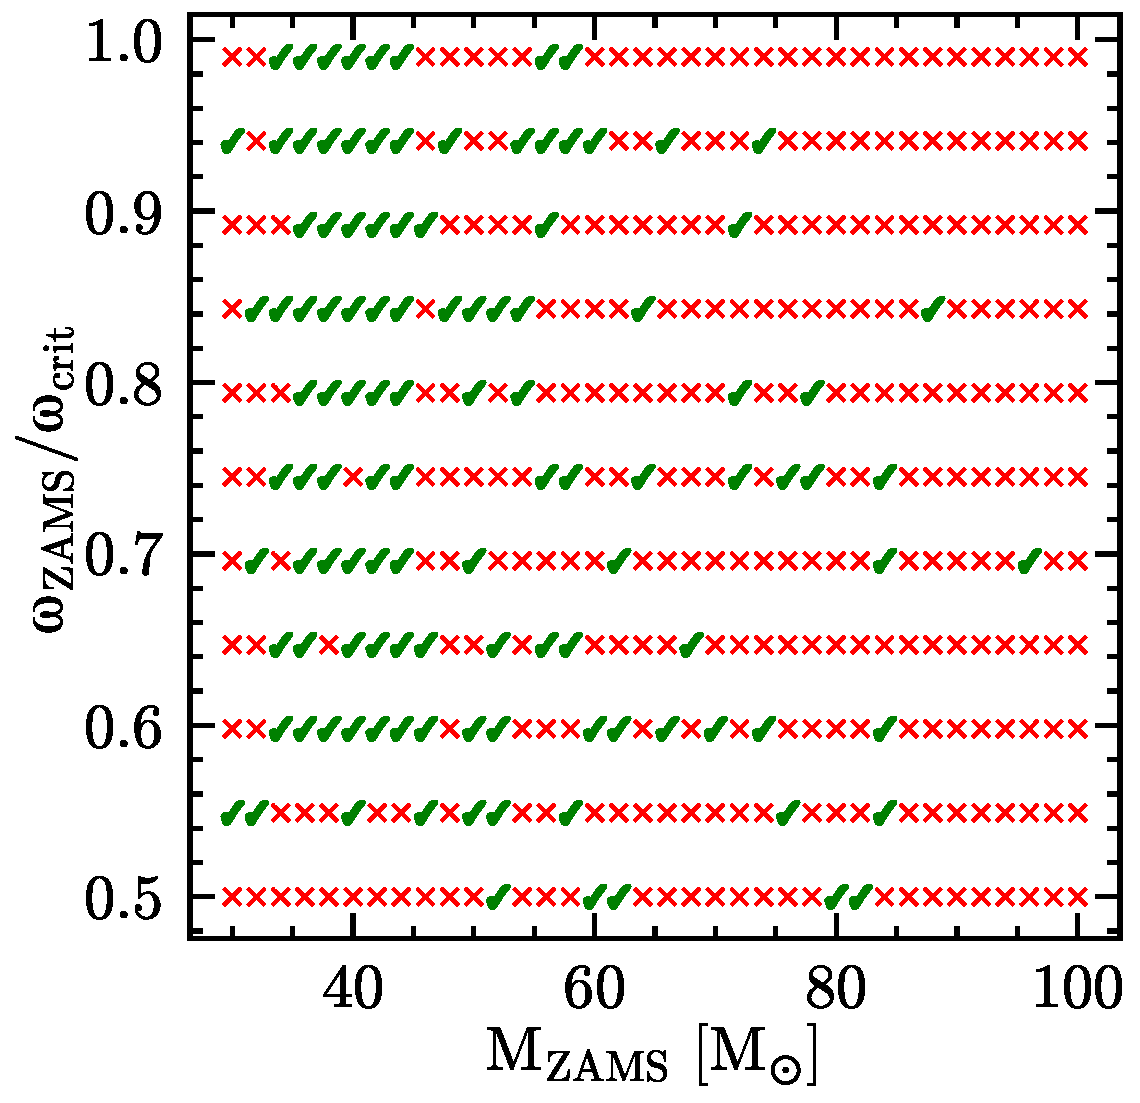
\includegraphics[width=0.5\textwidth]{figures/overview_grid}
  \caption{Overview of the grid success rate. Green check marks
    correspond to successful models. Red crosses correspond to models
    that either do not reach infall velocities of
    $-300\,\mathrm{km\ s^{-1}}$ or they exhibit large luminosity and
    effective temperature excursions that are treated un-physically in
    our setup and can impact the core-structure.}
  \label{fig:grid_success}
\end{figure}

Our grid consists initially of 11 values of
$\omega_{\rm ZAMS}/\omega_{\rm crit}$ per each of the 36
$M_{\rm ZAMS}$ values, for a total of 396 stellar models. Of these,
113 successfully reach the onset of core-collapse and pass our visual
inspection to remove models experiencing large $L$ and effective
temperature ($T_{\rm eff}$) excursions. These may be manifestations of
physical processes in the envelope \citep[e.g.,][for red-supergiant
stars]{heger:97} and/or numerical artifacts amplified by
the small timesteps necessary in late evolutionary phases (since the
acceleration term in the momentum equation is calculated as
$\Delta v/\Delta t$, it can become extremely large for small
$\Delta t$). Our setup is not designed to properly capture physical
phenomena in the outer envelopes this late in the evolution, and large
$L$ and $T_{\rm eff}$ can feedback on the core structure, motivating
our choice to exclude these models from our grid. Overall, our grid
has a 29\% success rate, relatively high for models that are
\emph{not} manually mentored in any way.

\begin{figure*}[htbp]
  \centering
  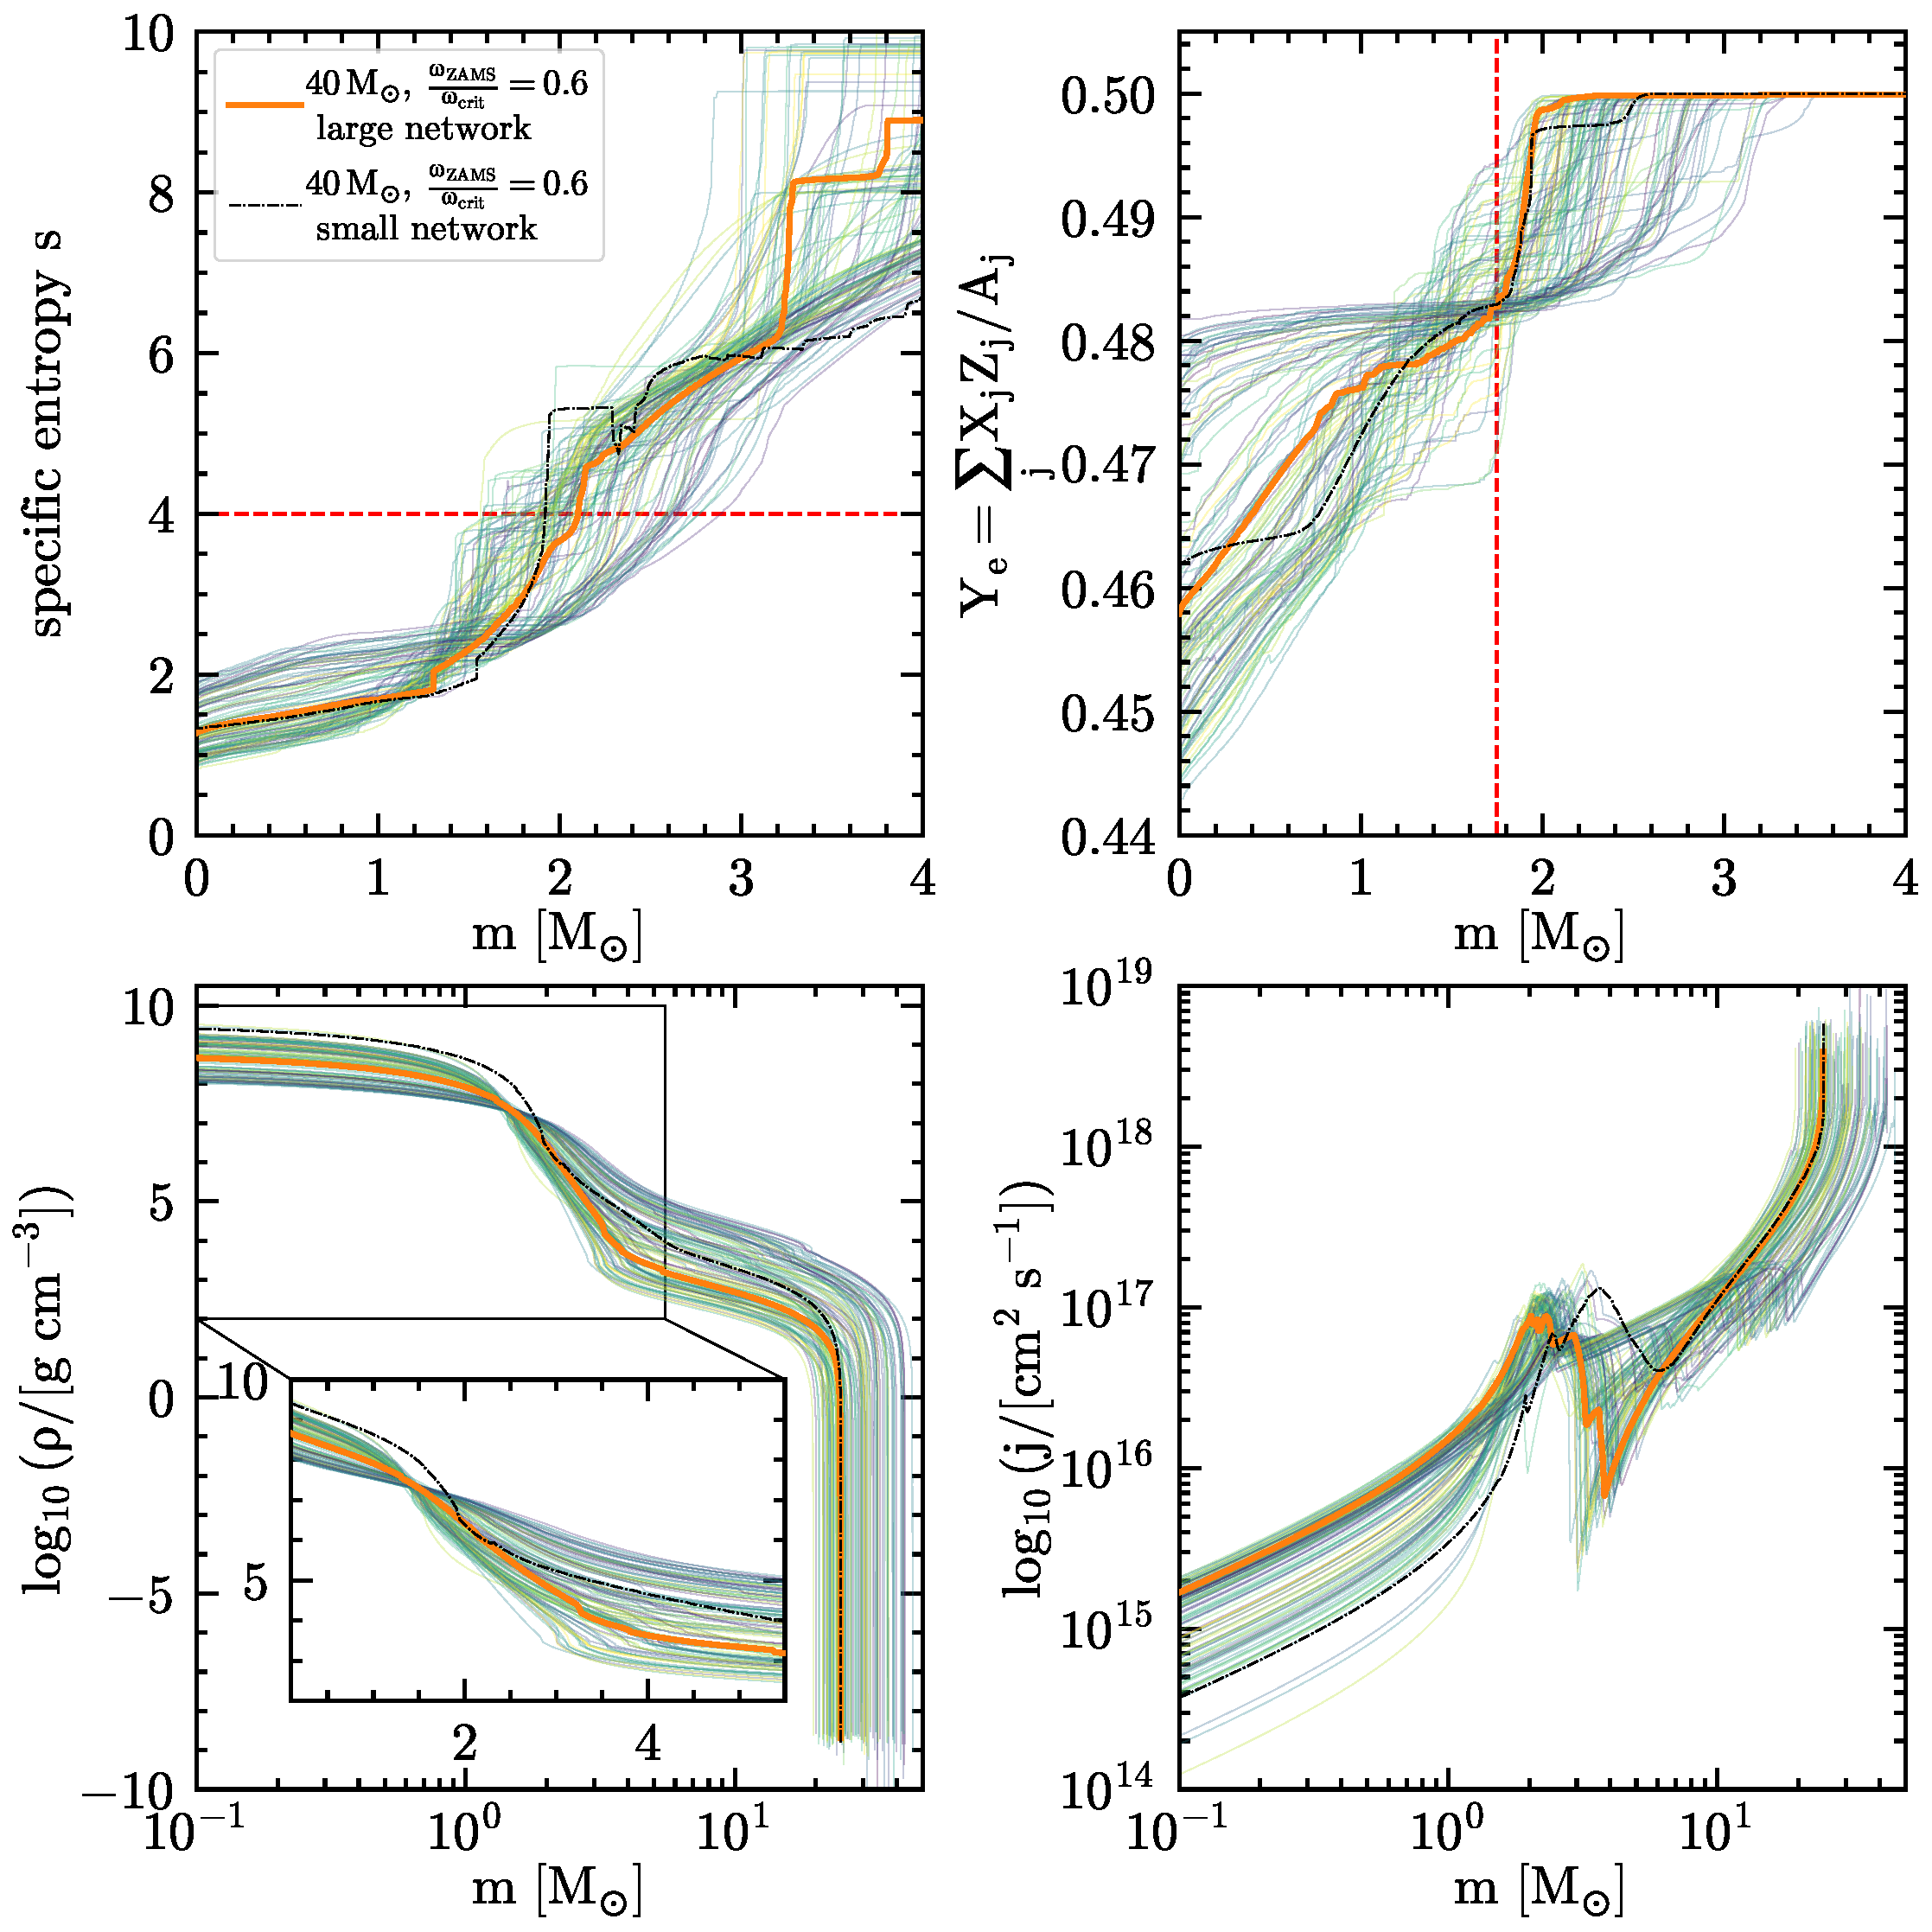
\includegraphics[width=\textwidth]{multipanel_grid.pdf}
  \caption{\emph{Top left}: Herzsprung-Russel diagram of
    rotationally-induced chemically-homogeneous evolving single star
    models. \emph{Top right:} Inner electron fraction $Y_{e}$ profile
    as a function of mass, the thin black dot-dashed line is the
    $40\,M_{\odot}$, $\omega_{\rm ZAMS}=0.6\,\omega_{\rm crit}$
    computed with a 22-isotope network from \cite{renzo:24} available
    from
    \href{https://doi.org/10.5281/zenodo.11375522}{10.5281/zenodo.11375522}.
    The vertical dashed line marks $\mathcal{M}=1.75\,M_{\odot}$ used
    to calculate the compactness $\xi_{1.75}$. \emph{Bottom left:}
    Density profiles as a function of Lagrangian mass coordinate $m$
    on a logarithmic scale. The inset zooms on the inner region and
    uses a linear scale. \emph{Bottom right:} Specific angular
    momentum profiles as a function of $m$. In all panels, the orange
    thick line marks a representative $40M_{\odot}$,
    $\omega_{\rm ZAMS}=0.6\,\omega_{\rm crit}$ used in
    \cite{gottlieb:24}.}
  \label{fig:multipanel}
\end{figure*}


As shown in \Figref{fig:grid_success}, successful models in our grid
sample relatively uniformly the parameter space
$30\,M_{\odot}\lesssim M_{\rm ZAMS}\lesssim 60\,M_{\odot}$ across all
rotation rates explored
($0.5\lesssim \omega_{\rm ZAMS}/\omega_{\rm crit}\lesssim 0.99$), and
the number of successes decrease at larger initial masses and rotation
rates. However, there is no particular threshold beyond which models
systematically fail: this suggests most failures come from numerical
errors in the solution of the stiff equations describing late stellar
evolution rather than physical hypothesis and/or their algorithmic
representation.

From this point onward, we focus on the analysis of the successful
models. \Figref{fig:multipanel} shows an overview of this grid, with
each thin blue line corresponding to one star. The thick
orange lines correspond to the model used as progenitor in
\cite{gottlieb:24}, highlighted to guide the eye.

The top left panel shows a Herzsprung-Russel diagram, where models
evolve from the bottom right towards the top left, as indicated by the
arrow. Because of the large rotation imposed at birth, these models
experience CHE (\citealt{maeder:00, yoon:06, demink:09}). Rotational
mixing (dominated by meridional circulations) prevents the formation
of a chemical stratification and the emergence of a core/envelope
boundary during the hydrogen-core burning main sequence. The entire
star is enriched in $^{4}\mathrm{He}$ (and $^{14}\mathrm{N}$ at the expenses of $^{12}\mathrm{C}$ and $^{16}\mathrm{O}$ because of the CNO cycle, \citealt{bethe:39}), reducing the envelope opacity
and preventing the red-ward evolution and radial expansion.
Nevertheless, the increase in mean-molecular weight leads to an
increase in luminosity \citep[e.g.,][]{kippenhahn:13, xin:2022}. % As noted in
% \cite{gottlieb:24}, with the large initial rotation assumed, the main
% sequence evolution leads to CHE even with the stronger angular
% momentum transport by \cite{fuller:19} and \cite{fuller:22}.

At the end of the hydrogen-core burning main sequence, each track
shows a characteristic ``hook'': this corresponds to a thermal
timescale phase of contraction because of the exhaustion of hydrogen
in the entire core region, corresponding to most of the star in this
CHE models.

Helium ignition in the center causes the star to briefly re-expand up
to its maximum radius. Nevertheless, each star remains relatively
small, with $\max(R)\lesssim 31\,R_{\odot}$ and
$T_{\rm eff}\gtrsim 10^{4.5}\,\mathrm{K}$ across the entire grid. This
minimizes the chances for binary mass-transfer with putative
companions for CHE stars \citep[e.g.,][]{demink:09}. We emphasize that
from this point onwards the evolution is not \emph{homogeneous}
anymore: while rotational mixing remains active, the evolutionary
timescale speeds up significantly owing to the lower energy release
per nucleon for heavier nuclear fuels, and chemical gradients seeded
by the burning impede further mixing \citep[e.g.,][]{heger:00,
  yoon:06, chieffi:13}. The stars develop a distinct carbon-oxygen
core, and a ``onion''-like structure.

The remaining evolution occurs roughly right-to-left at constant
luminosity, with wind mass-loss progressively removing mass, and
revealing hotter inner layers of the star. The hottest point and
smallest radius is reached roughly at core Neon ignition
\citep{gottlieb:24}, after which stars typically expand slightly
again. We note that the majority of the models failing (red crosses in
\Figref{fig:grid_success}, excluded from \Figref{fig:multipanel} and
beyond) occur during or after Neon core burning. This is because this
burning phase occurs through photodisintegration
$^{20}\mathrm{Ne}(\gamma, \alpha)^{16}\mathrm{O}$ which produces
$\alpha$ particles which have extremely high reaction rates at the
temperatures ($T \gtrsim 1.5\times10^{9}\,\mathrm{K}$,
\citealt{kippenhahn:13}), and thus the equations for the evolution of
the core composition become significantly stiffer and numerically
challenging.

The top right panel of \Figref{fig:multipanel} shows the profiles of
the electron fraction $Y_{e}=\sum_{j}X_{j}Z_{j}/A_{j}$, where $X_{j}$
is the mass fraction of the $j$-th isotope with charge $+Z_{j}e$ and
atomic mass $A_{j}$, in the innermost $m\le4\,M_{\odot}$ at
the onset of core-collapse. Outside
this mass coordinate $Y_e\simeq0.5$, while inside, weak-reactions, treated explicitly our nuclear reaction network, lead to
deleptonization and lower the $Y_{e}$ creating a profile consistent
with the thermodynamical conditions in the evolving cores. We also
show with a thin black dot-dashed line the $40\,M_{\odot}$,
$\omega_{\rm ZAMS}=0.6\,\omega_{\rm crit}$ model from \cite{renzo:24}
computed with a small 22-isotope network and an otherwise identical
setup, for comparison with the thick solid orange line corresponding
to the same initial conditions in our grid using a 128-isotope
network. The difference between these two $Y_{e}$ profiles is larger
than the difference between models of varying mass and initial
rotations: the systematic error from using a small nuclear reaction
network biases conclusions on the connection between progenitors,
explosions, and remnants \citep{farmer:16, renzo:24}.

In \Figref{fig:multipanel}, the bottom left panel shows the full
density profiles at the onset of collapse as a function of
$\log_{10}(m/M_{\odot})$, to focus on the inner layers of our CHE
models. The inset panel shows the innermost $m<5\,M_{\odot}$ on a
linear scale. The density profile $\rho(m)$ in these inner layers
depends strongly on the $Y_{e}(m)$ because of the contribution of
electron degeneracy pressure to the support of the core, and it
determines the infall velocity profile once electron-captures (and
later photodisintegration) remove pressure support
\citep[e.g.,][]{janka:12}. Moreover, the density determines the
initial accretion onto the shock generated at core-bounce, and thus
the neutrino luminosity \citep[e.g.][]{vartanyan:21, burrows:24}.
Finally, the density profile is also related to the angular momentum
profile via the mass-continuity equation relating $\rho(m)$ and the
radial distribution of mass $r(m)$.

The bottom right panel shows the specific angular momentum per unit
mass $j=r^{2}\omega$ at the onset of core-collapse. This can be
compared to the angular momentum of the innermost stable circular
orbit of a putative seed BH to decide whether a disk will form at
collapse \cite[e.g.,][]{macfadyen:94, perna:18}, or whether
a fast-spinning magnetar needs to form first \citep[e.g.,][]{kasen:10,
  gottlieb:24}.

\begin{figure}[htbp]
  \centering
  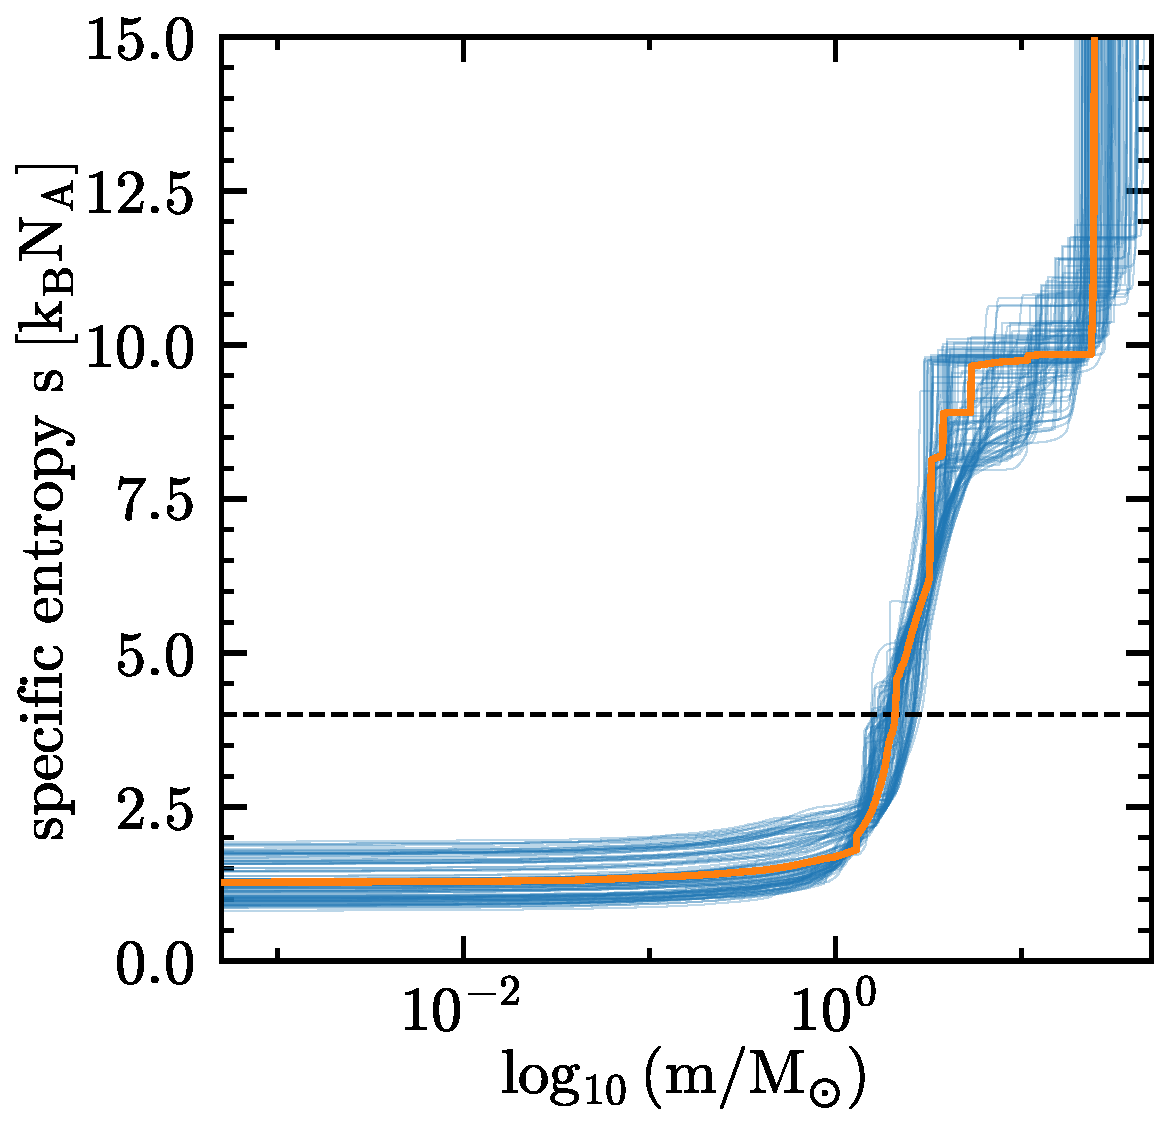
\includegraphics[width=0.5\textwidth]{entropy_grid}
  \caption{Specific entropy profiles. The dashed black horizontal line
    marks the $s=4\,k_{B}N_{A}$ location often used in
    ``explodability'' criteria \cite[e.g.,][]{ertl:16, ertl:20}. The orange
    thick line shows the $40M_{\odot}$,
    $\omega_{\rm ZAMS}=0.6\,\omega_{\rm crit}$ model from \cite{gottlieb:24}.}
  \label{fig:entropy}
\end{figure}

An alternative way to characterize the structure of our models at the
onset of core collapse is to look at the specific entropy profiles
$s$, presented in \Figref{fig:entropy}. Flat ``steps'' correspond to
stellar regions that experience \emph{efficient} convection, resulting
in a very-nearly adiabatic (i.e., constant $s$) profiles. The
mass-location of these depends on the detailed evolution of each
stellar model in our grid. \Figref{fig:entropy} vertical axis is cut
at $s=15\,k_{B}N_{A}$ to focus the visualization on the inner core
where stellar explosions are decide, and thus excludes the outer
(higher-entropy) layers of the stars.


\begin{figure}[tbp]
  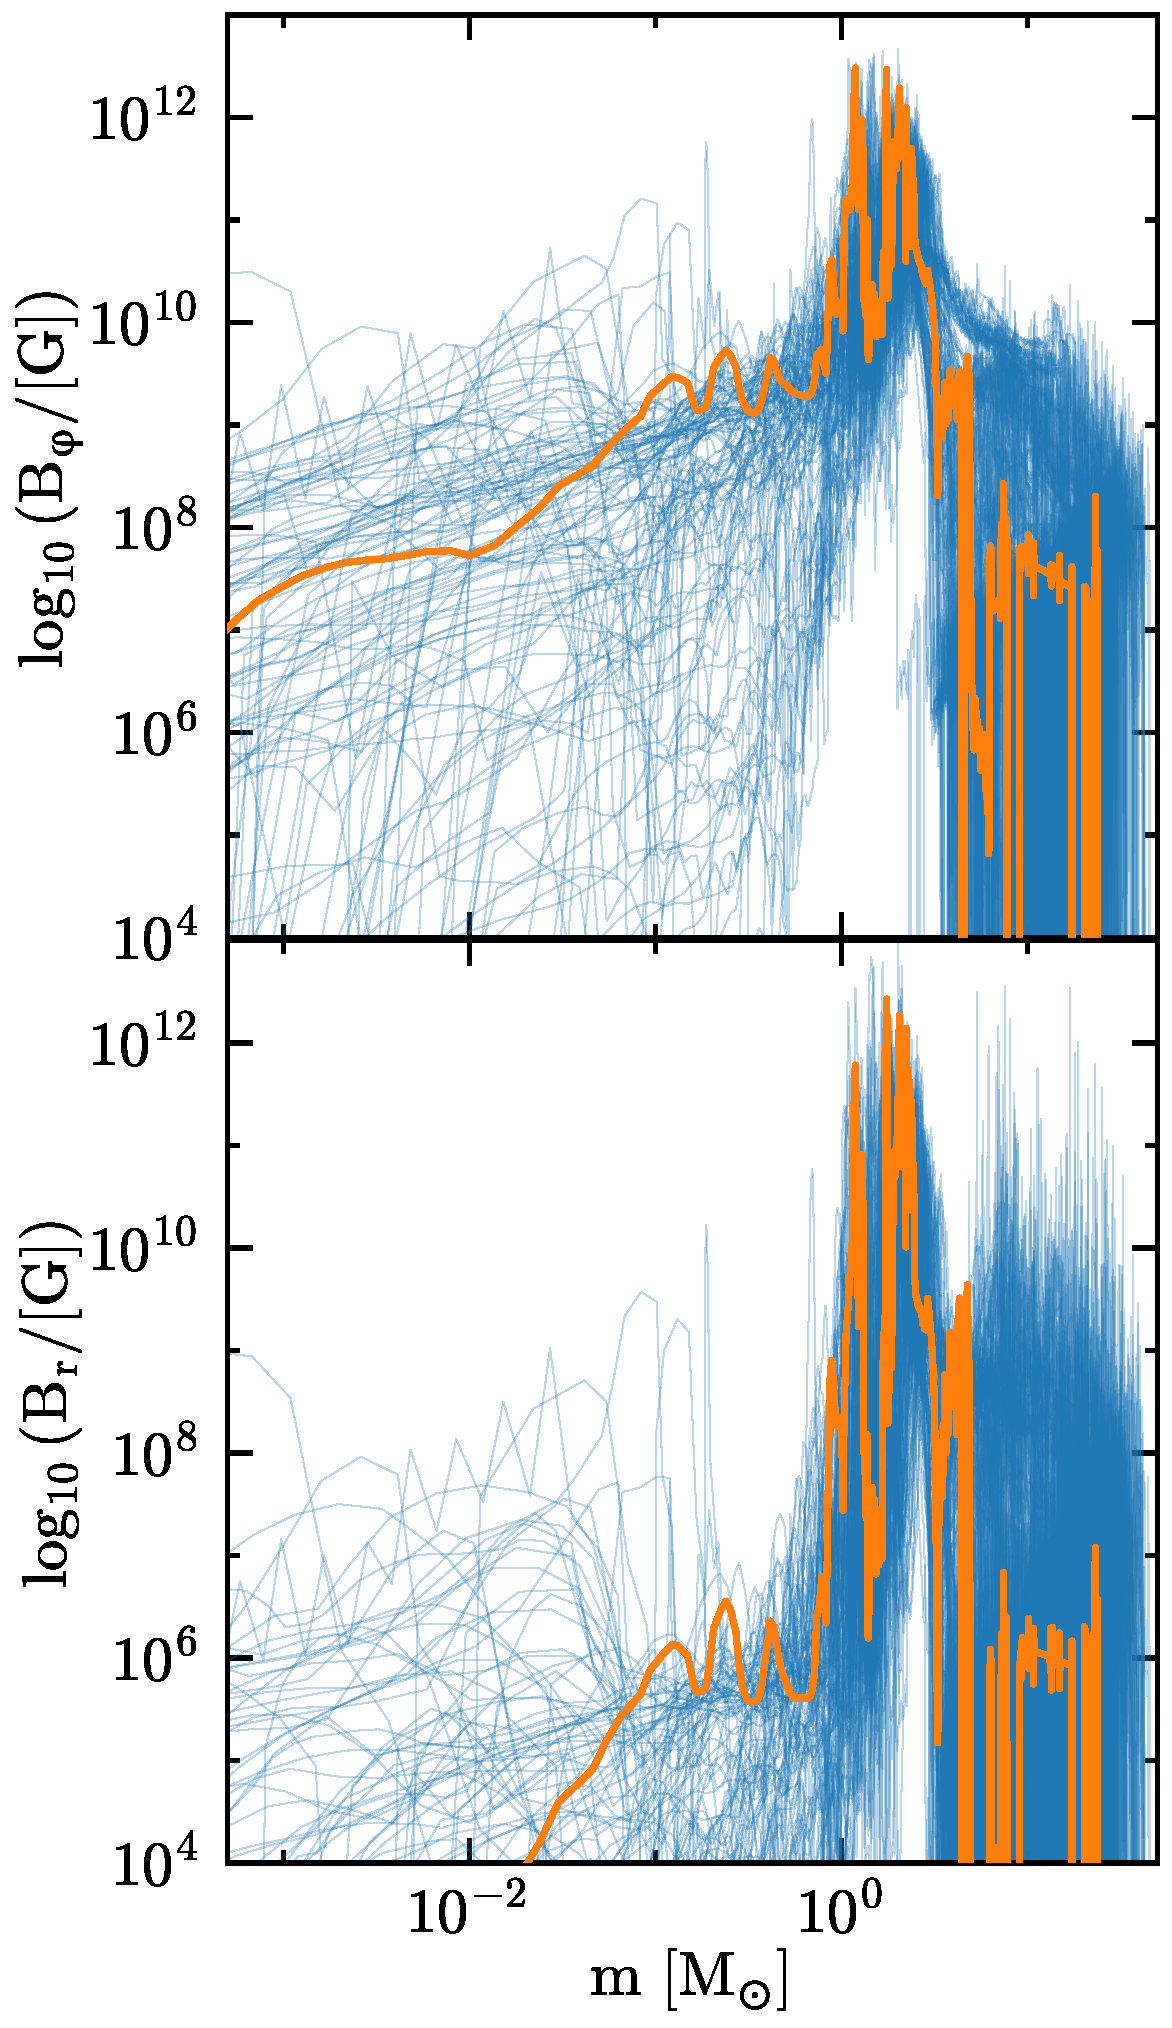
\includegraphics[width=0.5\textwidth]{B_phi_grid}
  \caption{Azimuthal (top) and radial (bottom) component of the
    \emph{local} magnetic field generated by the Spruit-Tayler dynamo
    as a function of Lagrangian mass coordinate. The orange thick line
    shows the $40M_{\odot}$, $\omega_{\rm ZAMS}=0.6\,\omega_{\rm crit}$
    model from \cite{gottlieb:24}.}
  \label{fig:B}
\end{figure}

The Tayler-Spruit dynamo responsible for angular momentum transport in
radiative regions of our CHE models generates magnetic fields.
\Figref{fig:B} shows the azimuthal ($B_\varphi$, top) and the radial
($B_{r}$, bottom) components as a function of mass coordinate on a
logarithmic scale at the onset of collapse. These magnetic fields are
\emph{local} and not large-scale coherently organized fields. We refer
interested readers to \cite{gottlieb:24} (Sec.~2.1) for more details
and how to calculate the magnetic flux advected during the initial
phases of a core collapse.


\begin{figure}[tbp]
  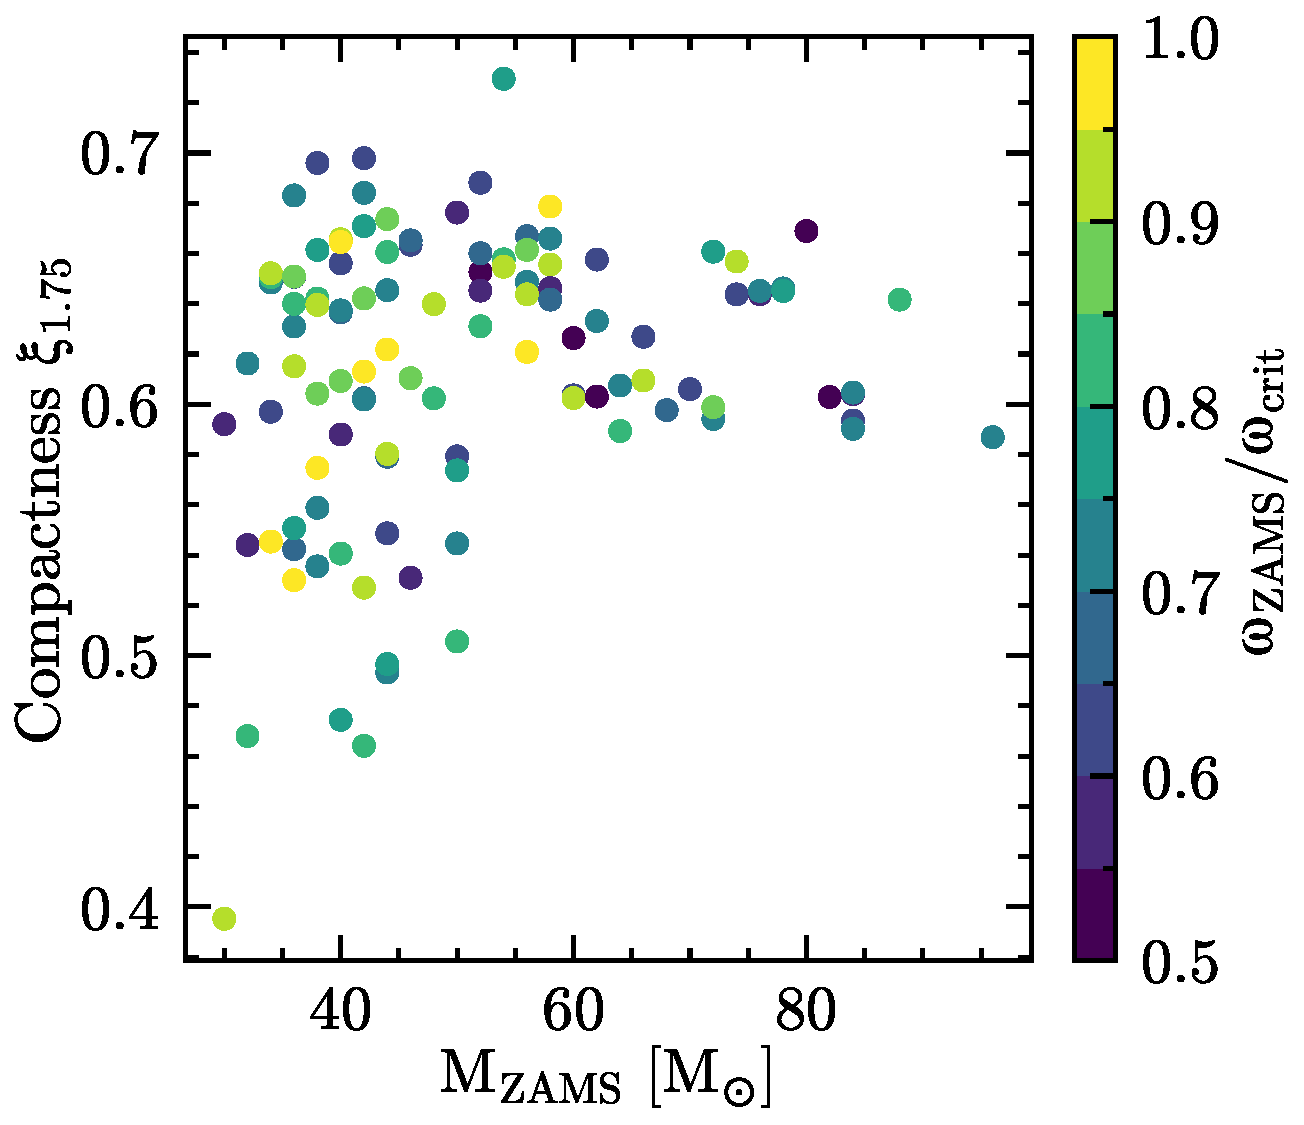
\includegraphics[width=0.5\textwidth]{xi_M}
  \caption{Compactness as a function initial mass and rotation rate for single CHE models. \todo{make Mzams top axis and Mfe bottom axis}}
  \label{fig:xi_M}
\end{figure}

\Figref{fig:xi_M} shows the compactness parameter \citep{oconnor:11}:
\begin{equation}
  \label{eq:compactness}
  \xi_{\mathcal{M}}=\frac{\mathcal{M}/M_{\odot}}{r(\mathcal{M})/1000\,\mathrm{km}} \ \ ,
\end{equation}
against the initial mass ($M_{\rm ZAMS}$, top axis) and iron core mass
($M_{\rm Fe}$, bottom axis), defined as the outermost location where
the mass fraction $X(^{28}\mathrm{Si})<0.1$ and $\sum_{j} X_{j}>0.1$
where the sum runs over all species with $A_{j}>46$. We use
$\mathcal{M}=1.75\,M_{\odot}$ to calculate the compactness following
\cite{burrows:24}, highlighted also by the vertical black dashed line
in the top right panel of \Figref{fig:multipanel}. Large values of
$\xi_{1.75}$ are more likely to result in BH formation, but this does
not imply the collapse does not result in a successful explosion since
the accretion rate on the shock, and consequently the neutrino
luminosity thought to drive the shock correlate positively with
$\xi_{1.75}$ \cite[e.g.,][]{kuroda:18, ott:18, burrows:25}.

The colors in \Figref{fig:xi_M} indicate the initial rotation rate,
and we see the typical correlation between iron core-mass and
compactness found in non-rotating models \citep[e.g.,][]{sukhbold:16,
  limongi:18}. Rotation introduces perturbations on this trend, and it
appears that initially faster rotating models (darker points) tend to
have a larger $\xi_{1.75}$, but this trend is not true at all masses
-- likely because of the high non-linearity of stellar evolution.

\section{Discussion}
\label{sec:discussion}

\subsection{What astrophysical scenario can these model represent?}
\label{sec:scenario}

The existence of direct observational evidence (e.g., from stellar
spectroscopy) for rotationally-induced chemically-homogeneous
evolution is still debated, although this evolutionary path becomes
more likely at very high stellar masses and low metallicities
\citep[e.g.,][]{yoon:06}. To produce fast-rotating collapsar
progenitors, we construct our stellar models at $Z=0.001$ and
\emph{assuming} extremely fast initial rotation rates. These are
prohibitively rare regardless of $Z$ in in young massive star
populations the local Universe \citep[e.g.,][]{hunter:08,
  ramirez-agudelo:13, ramirez-agudelo:15, dufton:19, galan-dieguez:26,
  lennon:26}. While there is growing evidence for relatively fast
($\gtrsim 250\,\mathrm{km\ s^{1}}$) primordial rotation
\citep[e.g.,][]{naze:23, britavskiy:24, naze:25}, these still have
$\omega\lesssim 0.3-0.4\,\omega_{\rm crit}$ and are not as fast as we
are assuming here. The fastest-rotating known O-type stars reach
$v\sin(i)\sim600\,\mathrm{km\ s^{-1}}$, likely in the regime
considered here, and are most likely accretor stars in interacting
binaries \citep{cantiello:07, ramirez-agudelo:15, renzo:21}. The
accretion process can change the core-envelope boundary in ways that
are not accounted for in our single-star models
\citep[e.g.,][]{cantiello:07, renzo:21, renzo:23, wagg:24, shah:26}.

/Nevertheless, the observation of jetted explosions and lGRBs suggest
that somehow, some stars reach core collapse with sufficient angular
momentum to form accretion disks onto a seed compact object. This
could be the product of accretion on the secondary in an interacting
binary system \citep[e.g.,][]{cantiello:07}, stellar mergers retaining
angular momentum \citep[e.g.,][]{chatzopoulos:20,renzo:20c}, tidal
spin up in post-common envelope massive binaries
\cite{bavera:20,bavera:22,sen:25}, or possibly inefficient angular
momentum transport in stars, leading to spin up of the core as it
evolves and contracts. We do not consider here the possibility of disk
formation from stochastic angular momentum in extended convective
envelopes \citep[e.g.,][]{quataert:19, shishkin:21,antoni:25} because
lGRBs are associated to type Ic broad-line SNe that require
hydrogen-free progenitors with compact envelopes.

We do not attempt to investigate the detailed evolutionary scenarios
leading to fast rotating cores. Instead, we provide a computationally
homogeneous grid of single, initially fast-rotating stellar
progenitors that could \emph{approximate} these scenarios in the hope
of enabling controlled numerical experiments for stellar collapse
where rotation and magnetic field are expected to play a role.


\subsection{Known physical and numerical caveats}
\label{sec:discussion_inputs}
The specific angular momentum profile of our models is a product of
the assumed initial rotation and the interplay between wind-mass loss
and angular momentum transport. We assumed a combination of
\cite{vink:00, vink:01} and \cite{nugis:00} for line-driven wind mass
loss, as opposed to most previous grids of fast-rotating progenitors
adopting a combination of \cite{nieuwenhuijzen:90}
\citep[e.g.,][]{woosley:06} and \cite{hamann:95}
\citep[e.g.,][]{aguilera-dena:18, aguilera-dena:20} . For angular
momentum transport, we adopt a Tayler-Spruit dynamo in radiative
regions \citep{spruit:02}. As noted in \cite{gottlieb:24} based on the
$40\,M_{\odot}$ model with $\omega_{\rm ZAMS}=0.6\,\omega_{\rm crit}$ (orange line in \Figref{fig:multipanel}-\ref{fig:B}),
adopting the stronger magnetic field saturation of the Tayler-Spruit
instability suggested in \cite{fuller:19, fuller:22} results in
slowly-rotating cores at collapse that do not produce accretion disks.
All these processes are highly uncertain in stellar context (see,
e.g., \citealt{smith:14, renzo:17, romagnolo:26} for wind-related
uncertainties, \citealt{spruit:99, cantiello:14, fuller:19,
  denhartogh:20, skoutnev:24, skoutnev:25} for angular momentum
transport uncertainties), and active topics of research.

The 128-isotope nuclear reaction network we adopt is sufficient to
resolve the density structure of the core. Increasing further the
network size has negligible impact on the electron fraction $Y_{e}$.
This has been shown both with full stellar models calculations
\citep[e.g.,][]{farmer:16} and focused one-zone experiments
\citep[e.g.,][]{grichener:25}. We note however that the list of
isotopes adopted here may still under-resolve the pre-collapse
neutrino flux \citep[e.g.,][]{farag:20} and may not be suitable for
detailed nucleosynthesis studies \citep[e.g.,][]{myers:26}.

Moreover, the nuclear reaction rates adopted (specifically the
$^{12}\mathrm{C}(\alpha,\gamma)^{16}\mathrm{O}$ from
\citealt{kunz:02}) are under active scrutiny in the community
\citep[e.g.,][]{deboer:17, takahashi:18, farmer:19, costa:21, shen:23,
  noll:25, tong:26} and our choice certainly influences the
pre-collapse structures presented here (like any other stellar models
in the literature).


As any set of stellar evolution calculations, the representation of
the inherently three-dimensional convective flow
\cite[e.g.,][]{jermyn:22,joyce:23} and convective boundaries
\cite[e.g.,][]{davis:19, myers:26} are potential causes of concern.
The key hypothesis of subsonic flows holds throughout the
evolution of our models. However, our choice of free parameters
($\alpha_{\rm MLT}$ and $\alpha_{\rm ov}$) to match existing
literature \citep[e.g.,][]{brott:11, aguilera-dena:18,
  aguilera-dena:20} may not be appropriate for every convective layer
in the stars \citep[e.g.,][]{griffiths:26}, and does not include the
latest updates from stellar hydrodynamics simulations
\citep[e.g.][]{anders:22, rizzuti:23, johnston:24}.

Maybe more importantly, our models adopt an artificial strategy to
expunge envelope velocities in the outer layers, possibly seeded by
numerical noise in the fast-paced late burning evolution. Significant
efforts to improve \textsc{MESA} to address these is ongoing.

Despite these inevitable caveats when producing numerical models
relying on input physics and physical processes under active
investigation, our models provide a significant update in the context
of fast-rotating CHE stars evolved until the onset of core-collapse.


\section{Conclusion}\label{sec:conclusion}

We presented a grid of rotationally-driven chemically-homogeneously
evolving massive stars at the onset of core-collapse. We have
described their evolution on the Herzsprung-Russel diagram and
characterized their internal profiles at the onset of core-collapse,
and discussed physical and numerical limitations of our calculations.

The evolution of these initially fast-rotating models represents
directly a presumably extremely rare evolutionary path based on
observations of initial rotation rates in the local Universe and rates
of astrophysical transients, and could approximate to a certain degree
more common evolutionary paths where rotation is produced, for
example, by binary interactions. Further studies to compare the
outcome of these pathways with single-fast rotating models are
necessary.

Despite the inevitable algorithmic and input physics limitations
inherent in numerical models (especially of astrophysical systems
represented by very stiff sets of equations), our models constitutes a
significant update in input physics and numerical accuracy for
fast-rotating collapsing stellar progenitors. We hope that our
publicly available results (at
\href{https://doi.org/10.5281/zenodo.14286306}{doi.org/10.5281/zenodo.14286306})
will be adopted for numerical experiments in studying the explosions
of rotating massive stars.\\


\software{This study made use of the following software packages: \textsc{MESA} \citep{paxton:11, paxton:13, paxton:15, paxton:19, jermyn:23},
 \texttt{python}
  \citep{python}, \texttt{numpy} \citep{numpy}, and \texttt{matplotlib} \citep{Hunter:2007}. Software citation information aggregated using
  \texttt{\href{https://www.tomwagg.com/software-citation-station/}{The
      Software Citation Station}}
  \citep{software-citation-station-paper,software-citation-station-zenodo}.}


\begin{acknowledgements}
  MR is grateful to N.~Britavskyi for many inspiring conversations on
  stellar rotation and E.~Farag for invaluable insights on stellar
  modeling in general and late burning stages of massive stars in
  particular.
\end{acknowledgements}

\bibliographystyle{aasjournalv7}
\bibliography{CHE_GRB_progenitors.bib}

\appendix

\section{Explodability metrics and surface composition}
\label{sec:table}

\Tabref{tab:explodability} lists for each successful model in our grid
a few key quantities related to their ``explodability'' and their
surface composition. Specifically, we list $\xi_{1.75}$ and
$M_{\rm Fe}$ shown also in \Figref{fig:xi_M}, $M_{4}$ is the outermost
mass coordinate where the specific entropy is $s=4\,k_{B}N_A$ and the
mass-gradient at that location $\mu_{4}$, which together can be
combined in the two-parameter explodability criterion by
\cite{ertl:16, ertl:20}.

The last three columns provide the surface mass fractions of the most
abundant elements, which are Helium
$Y_{\rm surf}\equiv X_{\rm surf}(^{4}\mathrm{He})$, Carbon, and
Oxygen. These do not necessarily sum to 1 because of other isotopes
present in our calculations, and are presumably sensitive to the wind
mass-loss rates and mixing processes. Interestingly, most of our
models still retain significant amount of helium at the surface (plus,
some helium-rich material can appear in the core very late due to
photodisintegration of iron-group nuclei).

\begin{longtable}{lc|cccc|cc|cc|ccc}
  \caption{\label{tab:explodability}\added{Core masses}, explodability metrics, and final surface composition  for our CHE models. The first two columns give the initial ZAMS values of mass and initial rotational frequency in units of $\omega_{\rm crit}$. The following three columns give the final iron ($M_{\rm Fe}$), silicon ($M_{\rm Si}$), and carbon-oxygen core masses ($M_{\rm CO}$), defined as the outermost location where the mass fraction of an element (or their sum in the case of carbon and oxygen) rises above 0.1 and the mass fraction of the lighter element drops below 0.1. For the iron core, we consider $\sum_{j} X_{j}>0.1$  where the sum
  runs over all species with $A_{j}>46$. The next two columns
  gives the Helium core mass
  $M_{\rm He}$ and total mass $M$ at terminal age main sequence, defined as $X_{c}(^{1}\mathrm{H})\le10^{-2}$. Then we list the compactness parameter $\xi_{1.75}$ \citep{oconnor:11}
  calculated at mass coordinate $\mathcal{M}=1.75\,M_{\odot}$
  \citep{burrows:24},
  and the two parameters  $M_{4}\equiv\max(m(s<4\,k_{B}N_{A}))$ and  $\mu_{4}=dm/dr(m=M_{4})$
  for the \cite{ertl:16, ertl:20} explodability criterion. The last three columns are the final surface mass
  fractions of helium
  $Y_{\rm surf}\equiv X_{\rm surf}(^{4}\mathrm{He})$, carbon, and
  oxygen. These do not necessarily sum to 1 because of other isotopes
  present in our calculations.}\\

\hline
$M_{\rm ZAMS}$ & $\omega_{\rm ZAMS}$ & $M_{\rm Fe}$ & $M_{\rm Si}$ & $M_{\rm CO}$ & $M_{\rm He, TAMS}$ & $M_{\rm TAMS}$ & \multirow{2}{*}{$\xi_{1.75}$} & $M_{4}$ & $\mu_{4}$ & \multirow{2}{*}{$Y_{\rm surf}$} & \multirow{2}{*}{$X_{\rm surf}(^{12}\mathrm{C})$} & \multirow{2}{*}{$X_{\rm surf}(^{16}\mathrm{O})$} \\
$[M_{\odot}]$ & $[\omega_{\rm crit}]$ &  $[M_{\odot}]$ & $[M_{\odot}]$ & $[M_{\odot}]$ & $[M_{\odot}]$ & $[M_{\odot}]$ &  & $[M_{\odot}]$ & $[M_{\odot}/10^{3}\,\mathrm{km}]$ & & & \\
  \hline
  \hline
  \endfirsthead
  \hline
  \multicolumn{13}{c}{(continued from previous page)}\\
  \hline
  \hline
$M_{\rm ZAMS}$ & $\omega_{\rm ZAMS}$ & $M_{\rm Fe}$ & $M_{\rm Si}$ & $M_{\rm CO}$ & $M_{\rm He, TAMS}$ & $M_{\rm TAMS}$ & \multirow{2}{*}{$\xi_{1.75}$} & $M_{4}$ & $\mu_{4}$ & \multirow{2}{*}{$Y_{\rm surf}$} & \multirow{2}{*}{$X_{\rm surf}(^{12}\mathrm{C})$} & \multirow{2}{*}{$X_{\rm surf}(^{16}\mathrm{O})$} \\
$[M_{\odot}]$ & $[\omega_{\rm crit}]$ &  $[M_{\odot}]$ & $[M_{\odot}]$ & $[M_{\odot}]$ & $[M_{\odot}]$ & $[M_{\odot}]$ &  & $[M_{\odot}]$ & $[M_{\odot}/10^{3}\,\mathrm{km}]$ & & & \\
  \hline
  \hline
  \endhead
  % python output here
\hline
30.00 & 0.55 & 1.41 & 1.41 & 19.15 & 19.20 & 24.07 & 0.592 & 1.70 & 0.173 & 0.32 & 0.16 & 0.48\\
30.00 & 0.94 & 3.14 & 1.41 & 18.37 & 17.87 & 23.01 & 0.395 & 1.56 & 0.114 & 0.26 & 0.16 & 0.51\\
\hline
32.00 & 0.55 & 2.23 & 1.48 & 20.85 & 21.93 & 26.00 & 0.544 & 1.96 & 0.134 & 0.31 & 0.21 & 0.42\\
32.00 & 0.70 & 1.76 & 1.71 & 19.33 & 19.27 & 24.61 & 0.616 & 1.81 & 0.133 & 0.31 & 0.15 & 0.46\\
32.00 & 0.84 & 2.21 & 1.34 & 19.66 & 19.14 & 24.30 & 0.468 & 1.58 & 0.143 & 0.46 & 0.09 & 0.34\\
\hline
34.00 & 0.60 & 2.10 & 1.54 & 21.59 & 20.81 & 26.29 & 0.597 & 1.88 & 0.133 & 0.66 & 0.04 & 0.22\\
34.00 & 0.65 & 1.33 & 1.32 & 20.57 & 20.63 & 26.06 & 0.650 & 1.95 & 0.179 & 0.37 & 0.14 & 0.44\\
34.00 & 0.74 & 1.45 & 1.45 & 20.53 & 20.50 & 25.67 & 0.648 & 2.05 & 0.166 & 0.24 & 0.17 & 0.54\\
34.00 & 0.84 & 1.76 & 1.76 & 20.45 & 20.40 & 25.53 & 0.651 & 1.90 & 0.132 & 0.26 & 0.16 & 0.53\\
34.00 & 0.94 & 1.46 & 1.46 & 19.73 & 20.26 & 25.44 & 0.652 & 1.91 & 0.153 & 0.40 & 0.14 & 0.41\\
34.00 & 0.99 & 2.11 & 1.49 & 20.62 & 20.30 & 25.41 & 0.545 & 1.85 & 0.127 & 0.73 & 0.04 & 0.17\\
\hline
36.00 & 0.60 & 2.10 & 1.46 & 22.01 & 22.07 & 27.53 & 0.651 & 1.90 & 0.138 & 0.26 & 0.16 & 0.50\\
36.00 & 0.65 & 3.39 & 1.46 & 21.85 & 21.89 & 27.23 & 0.542 & 1.76 & 0.186 & 0.28 & 0.16 & 0.49\\
36.00 & 0.70 & 2.11 & 1.52 & 21.69 & 21.83 & 27.05 & 0.683 & 1.92 & 0.144 & 0.25 & 0.17 & 0.50\\
36.00 & 0.74 & 1.49 & 1.50 & 21.79 & 21.74 & 26.92 & 0.631 & 2.08 & 0.180 & 0.82 & 0.03 & 0.10\\
36.00 & 0.79 & 2.20 & 1.56 & 21.88 & 21.62 & 26.81 & 0.551 & 1.99 & 0.134 & 0.75 & 0.04 & 0.15\\
36.00 & 0.84 & 1.31 & 1.31 & 20.93 & 21.56 & 26.67 & 0.640 & 2.14 & 0.193 & 0.29 & 0.17 & 0.51\\
36.00 & 0.89 & 1.42 & 1.42 & 21.26 & 21.49 & 26.66 & 0.651 & 2.11 & 0.180 & 0.25 & 0.17 & 0.53\\
36.00 & 0.94 & 2.13 & 1.51 & 21.17 & 21.58 & 26.64 & 0.615 & 1.94 & 0.134 & 0.29 & 0.16 & 0.47\\
36.00 & 0.99 & 2.12 & 1.45 & 21.32 & 21.56 & 26.57 & 0.530 & 1.91 & 0.131 & 0.52 & 0.07 & 0.30\\
\hline
38.00 & 0.60 & 2.18 & 1.64 & 23.39 & 23.32 & 28.79 & 0.696 & 2.12 & 0.180 & 0.76 & 0.05 & 0.14\\
38.00 & 0.70 & 2.36 & 1.43 & 22.65 & 23.06 & 28.25 & 0.559 & 1.77 & 0.148 & 0.46 & 0.08 & 0.34\\
38.00 & 0.74 & 2.45 & 1.45 & 22.81 & 23.04 & 28.09 & 0.536 & 1.69 & 0.150 & 0.61 & 0.07 & 0.23\\
38.00 & 0.79 & 1.66 & 1.66 & 22.67 & 22.89 & 28.00 & 0.661 & 2.16 & 0.229 & 0.70 & 0.06 & 0.18\\
38.00 & 0.84 & 1.41 & 1.41 & 22.35 & 22.80 & 27.89 & 0.642 & 2.07 & 0.197 & 0.70 & 0.06 & 0.17\\
38.00 & 0.89 & 1.54 & 1.54 & 21.96 & 22.80 & 27.84 & 0.604 & 1.74 & 0.150 & 0.53 & 0.10 & 0.30\\
38.00 & 0.94 & 1.42 & 1.42 & 22.58 & 22.80 & 27.76 & 0.640 & 1.98 & 0.177 & 0.67 & 0.07 & 0.19\\
38.00 & 0.99 & 2.16 & 1.54 & 22.27 & 22.73 & 27.76 & 0.575 & 1.99 & 0.121 & 0.48 & 0.09 & 0.32\\
\hline
40.00 & 0.55 & 1.48 & 1.48 & 24.38 & 24.74 & 30.46 & 0.588 & 1.81 & 0.204 & 0.28 & 0.17 & 0.50\\
40.00 & 0.60 & 1.62 & 1.62 & 24.36 & 24.63 & 29.94 & 0.656 & 2.10 & 0.177 & 0.85 & 0.06 & 0.07\\
40.00 & 0.65 & 2.76 & 1.65 & 23.94 & 24.50 & 29.62 & 0.637 & 1.81 & 0.158 & 0.83 & 0.07 & 0.08\\
40.00 & 0.70 & 2.23 & 1.51 & 23.58 & 24.38 & 29.39 & 0.637 & 1.94 & 0.135 & 0.45 & 0.10 & 0.33\\
40.00 & 0.79 & 2.18 & 1.55 & 23.47 & 24.15 & 29.08 & 0.474 & 1.94 & 0.114 & 0.27 & 0.12 & 0.45\\
40.00 & 0.84 & 2.16 & 1.52 & 23.24 & 24.06 & 28.99 & 0.541 & 1.80 & 0.146 & 0.55 & 0.10 & 0.27\\
40.00 & 0.89 & 2.68 & 23.82 & 23.34 & 24.08 & 28.96 & 0.609 & 1.61 & 0.218 & 0.90 & 0.07 & 0.03\\
40.00 & 0.94 & 1.49 & 1.49 & 23.43 & 23.99 & 28.91 & 0.666 & 2.07 & 0.178 & 0.71 & 0.09 & 0.16\\
40.00 & 0.99 & 1.37 & 1.37 & 23.40 & 24.01 & 28.90 & 0.665 & 2.08 & 0.181 & 0.88 & 0.07 & 0.04\\
\hline
42.00 & 0.60 & 1.72 & 1.72 & 25.12 & 26.00 & 31.06 & 0.698 & 2.00 & 0.186 & 0.73 & 0.11 & 0.14\\
42.00 & 0.65 & 1.59 & 1.59 & 24.82 & 25.74 & 30.80 & 0.602 & 2.14 & 0.147 & 0.84 & 0.11 & 0.05\\
42.00 & 0.70 & 2.07 & 1.77 & 24.53 & 25.67 & 30.53 & 0.602 & 1.88 & 0.135 & 0.34 & 0.15 & 0.41\\
42.00 & 0.74 & 1.81 & 1.81 & 24.57 & 25.48 & 30.44 & 0.684 & 1.88 & 0.178 & 0.74 & 0.11 & 0.12\\
42.00 & 0.79 & 1.89 & 1.89 & 24.39 & 25.48 & 30.24 & 0.671 & 2.18 & 0.211 & 0.77 & 0.11 & 0.10\\
42.00 & 0.84 & 2.16 & 1.40 & 24.39 & 25.36 & 30.13 & 0.464 & 1.74 & 0.143 & 0.44 & 0.12 & 0.33\\
42.00 & 0.89 & 1.58 & 1.58 & 24.16 & 25.29 & 30.03 & 0.642 & 2.04 & 0.197 & 0.78 & 0.11 & 0.09\\
42.00 & 0.94 & 2.32 & 1.45 & 24.25 & 25.31 & 30.03 & 0.527 & 1.72 & 0.162 & 0.67 & 0.11 & 0.17\\
42.00 & 0.99 & 2.08 & 1.58 & 23.77 & 25.31 & 30.01 & 0.613 & 1.91 & 0.138 & 0.44 & 0.13 & 0.33\\
\hline
44.00 & 0.60 & 2.18 & 1.50 & 26.07 & 27.27 & 32.31 & 0.549 & 1.77 & 0.150 & 0.37 & 0.15 & 0.38\\
44.00 & 0.65 & 2.17 & 1.46 & 25.58 & 27.12 & 31.93 & 0.579 & 1.93 & 0.131 & 0.40 & 0.15 & 0.35\\
44.00 & 0.70 & 2.41 & 1.00 & 25.47 & 26.94 & 31.67 & 0.493 & 1.68 & 0.140 & 0.63 & 0.15 & 0.18\\
44.00 & 0.74 & 1.37 & 1.37 & 25.31 & 26.79 & 31.51 & 0.645 & 2.07 & 0.190 & 0.79 & 0.15 & 0.06\\
44.00 & 0.79 & 2.21 & 1.49 & 25.22 & 26.69 & 31.35 & 0.497 & 1.95 & 0.134 & 0.46 & 0.15 & 0.31\\
44.00 & 0.84 & 2.02 & 2.02 & 25.02 & 26.62 & 31.27 & 0.661 & 2.13 & 0.236 & 0.78 & 0.15 & 0.07\\
44.00 & 0.89 & 2.77 & 1.33 & 25.17 & 26.54 & 31.16 & 0.674 & 1.74 & 0.205 & 0.69 & 0.15 & 0.14\\
44.00 & 0.94 & 1.44 & 1.44 & 25.05 & 26.49 & 31.14 & 0.580 & 1.95 & 0.148 & 0.38 & 0.15 & 0.37\\
44.00 & 0.99 & 2.10 & 1.58 & 24.98 & 26.52 & 31.12 & 0.622 & 1.87 & 0.145 & 0.39 & 0.15 & 0.35\\
\hline
46.00 & 0.55 & 1.75 & 1.75 & 27.21 & 28.91 & 33.86 & 0.531 & 1.94 & 0.141 & 0.53 & 0.17 & 0.24\\
46.00 & 0.60 & 1.95 & 1.95 & 26.89 & 28.53 & 33.42 & 0.664 & 2.05 & 0.226 & 0.73 & 0.18 & 0.08\\
46.00 & 0.65 & 2.83 & 1.89 & 26.33 & 28.38 & 33.06 & 0.665 & 1.96 & 0.199 & 0.75 & 0.18 & 0.07\\
46.00 & 0.89 & 2.21 & 1.81 & 25.99 & 27.78 & 32.27 & 0.610 & 1.88 & 0.148 & 0.40 & 0.17 & 0.34\\
\hline
48.00 & 0.84 & 1.39 & 1.39 & 26.52 & 29.07 & 33.47 & 0.602 & 1.92 & 0.164 & 0.54 & 0.21 & 0.21\\
48.00 & 0.94 & 1.38 & 1.38 & 26.62 & 28.98 & 33.29 & 0.640 & 1.88 & 0.177 & 0.47 & 0.19 & 0.27\\
\hline
50.00 & 0.55 & 1.50 & 1.50 & 28.42 & 31.43 & 36.07 & 0.676 & 2.01 & 0.199 & 0.62 & 0.26 & 0.12\\
50.00 & 0.60 & 1.26 & 1.26 & 28.42 & 31.15 & 35.62 & 0.579 & 2.03 & 0.149 & 0.54 & 0.23 & 0.19\\
50.00 & 0.70 & 2.33 & 1.02 & 28.05 & 30.68 & 34.98 & 0.545 & 1.58 & 0.176 & 0.52 & 0.22 & 0.22\\
50.00 & 0.79 & 2.30 & 1.40 & 27.90 & 30.39 & 34.66 & 0.574 & 1.89 & 0.154 & 0.56 & 0.23 & 0.18\\
50.00 & 0.84 & 1.36 & 1.36 & 27.75 & 30.28 & 34.54 & 0.506 & 1.62 & 0.155 & 0.52 & 0.22 & 0.21\\
\hline
52.00 & 0.50 & 1.59 & 1.59 & 30.15 & 33.28 & 37.72 & 0.653 & 2.04 & 0.201 & 0.57 & 0.29 & 0.13\\
52.00 & 0.55 & 1.60 & 1.60 & 29.68 & 32.77 & 37.20 & 0.645 & 2.23 & 0.204 & 0.59 & 0.28 & 0.12\\
52.00 & 0.60 & 1.81 & 1.81 & 29.22 & 32.39 & 36.73 & 0.688 & 2.20 & 0.199 & 0.61 & 0.27 & 0.11\\
52.00 & 0.65 & 2.02 & 2.01 & 28.88 & 32.16 & 36.32 & 0.660 & 2.26 & 0.263 & 0.63 & 0.26 & 0.11\\
52.00 & 0.84 & 2.31 & 1.53 & 28.37 & 31.54 & 35.55 & 0.631 & 2.00 & 0.153 & 0.40 & 0.23 & 0.31\\
\hline
54.00 & 0.79 & 1.79 & 1.79 & 29.32 & 32.81 & 36.74 & 0.730 & 1.97 & 0.194 & 0.37 & 0.27 & 0.32\\
54.00 & 0.84 & 2.09 & 2.09 & 29.38 & 32.69 & 36.61 & 0.658 & 2.18 & 0.248 & 0.31 & 0.27 & 0.36\\
54.00 & 0.94 & 1.48 & 1.47 & 29.27 & 32.47 & 36.48 & 0.655 & 1.96 & 0.195 & 0.54 & 0.27 & 0.17\\
\hline
56.00 & 0.65 & 2.81 & 2.46 & 30.73 & 34.60 & 38.47 & 0.667 & 2.49 & 0.277 & 0.29 & 0.29 & 0.37\\
56.00 & 0.74 & 2.12 & 2.12 & 30.40 & 34.16 & 38.00 & 0.649 & 2.29 & 0.260 & 0.38 & 0.29 & 0.30\\
56.00 & 0.89 & 2.09 & 2.09 & 29.98 & 33.80 & 37.54 & 0.661 & 2.24 & 0.249 & 0.39 & 0.29 & 0.29\\
56.00 & 0.94 & 1.42 & 1.42 & 30.01 & 33.71 & 37.50 & 0.644 & 1.96 & 0.185 & 0.44 & 0.27 & 0.25\\
56.00 & 0.99 & 2.07 & 2.07 & 29.98 & 33.74 & 37.45 & 0.621 & 2.34 & 0.268 & 0.45 & 0.30 & 0.24\\
\hline
58.00 & 0.55 & 2.33 & 1.69 & 32.09 & 36.61 & 40.38 & 0.646 & 2.24 & 0.186 & 0.54 & 0.33 & 0.13\\
58.00 & 0.65 & 2.11 & 2.11 & 31.62 & 35.81 & 39.51 & 0.642 & 2.63 & 0.340 & 0.42 & 0.31 & 0.24\\
58.00 & 0.74 & 2.01 & 2.01 & 31.10 & 35.41 & 38.99 & 0.666 & 2.26 & 0.268 & 0.42 & 0.32 & 0.25\\
58.00 & 0.94 & 2.51 & 1.99 & 30.91 & 34.88 & 38.49 & 0.656 & 2.33 & 0.248 & 0.39 & 0.30 & 0.28\\
58.00 & 0.99 & 1.61 & 1.61 & 30.62 & 34.84 & 38.44 & 0.679 & 2.14 & 0.229 & 0.56 & 0.31 & 0.12\\
\hline
60.00 & 0.50 & 2.01 & 2.01 & 33.63 & 38.53 & 41.95 & 0.626 & 2.51 & 0.293 & 0.36 & 0.32 & 0.28\\
60.00 & 0.60 & 2.27 & 2.27 & 32.82 & 37.38 & 40.97 & 0.604 & 2.54 & 0.294 & 0.48 & 0.33 & 0.18\\
60.00 & 0.94 & 2.15 & 2.15 & 31.70 & 36.04 & 39.48 & 0.602 & 2.59 & 0.305 & 0.52 & 0.33 & 0.15\\
\hline
62.00 & 0.50 & 2.17 & 2.17 & 34.44 & 39.75 & 42.98 & 0.603 & 2.64 & 0.297 & 0.42 & 0.32 & 0.22\\
62.00 & 0.60 & 2.04 & 2.04 & 33.61 & 38.62 & 42.00 & 0.658 & 2.40 & 0.282 & 0.39 & 0.33 & 0.25\\
62.00 & 0.70 & 2.04 & 2.04 & 33.00 & 37.92 & 41.28 & 0.633 & 2.38 & 0.276 & 0.38 & 0.33 & 0.27\\
\hline
64.00 & 0.74 & 2.12 & 2.12 & 33.58 & 38.90 & 42.03 & 0.607 & 2.41 & 0.278 & 0.38 & 0.33 & 0.26\\
64.00 & 0.84 & 2.43 & 2.43 & 33.33 & 38.53 & 41.63 & 0.589 & 2.76 & 0.352 & 0.37 & 0.33 & 0.27\\
\hline
66.00 & 0.60 & 2.07 & 2.07 & 35.34 & 41.02 & 43.99 & 0.627 & 2.61 & 0.343 & 0.45 & 0.36 & 0.18\\
66.00 & 0.94 & 2.15 & 2.15 & 33.91 & 39.46 & 42.40 & 0.609 & 2.43 & 0.315 & 0.38 & 0.33 & 0.26\\
\hline
68.00 & 0.65 & 2.17 & 2.17 & 35.69 & 41.80 & 44.55 & 0.598 & 2.58 & 0.318 & 0.40 & 0.35 & 0.23\\
\hline
70.00 & 0.60 & 2.14 & 2.14 & 36.93 & 43.47 & 45.97 & 0.606 & 2.60 & 0.294 & 0.45 & 0.37 & 0.17\\
\hline
72.00 & 0.74 & 2.18 & 2.18 & 36.80 & 43.55 & 45.90 & 0.594 & 2.61 & 0.311 & 0.37 & 0.35 & 0.25\\
72.00 & 0.79 & 2.04 & 2.04 & 36.63 & 43.30 & 45.64 & 0.661 & 2.58 & 0.307 & 0.49 & 0.38 & 0.13\\
72.00 & 0.89 & 2.29 & 2.29 & 36.28 & 42.92 & 45.29 & 0.599 & 2.57 & 0.313 & 0.46 & 0.38 & 0.15\\
\hline
74.00 & 0.60 & 2.14 & 2.14 & 38.41 & 45.87 & 47.88 & 0.644 & 2.64 & 0.309 & 0.48 & 0.39 & 0.13\\
74.00 & 0.94 & 2.12 & 2.12 & 36.96 & 43.94 & 46.11 & 0.657 & 2.31 & 0.274 & 0.49 & 0.38 & 0.13\\
\hline
76.00 & 0.55 & 2.46 & 2.21 & 39.38 & 47.62 & 49.38 & 0.644 & 2.32 & 0.253 & 0.47 & 0.39 & 0.13\\
76.00 & 0.74 & 1.49 & 1.49 & 38.17 & 45.89 & 47.75 & 0.645 & 1.98 & 0.235 & 0.48 & 0.39 & 0.12\\
\hline
78.00 & 0.74 & 2.02 & 2.02 & 38.93 & 47.00 & 48.68 & 0.646 & 2.58 & 0.350 & 0.44 & 0.38 & 0.17\\
78.00 & 0.79 & 1.99 & 1.99 & 38.69 & 46.73 & 48.41 & 0.645 & 2.23 & 0.238 & 0.44 & 0.37 & 0.17\\
\hline
80.00 & 0.50 & 2.10 & 2.10 & 41.50 & 51.01 & 52.04 & 0.669 & 2.32 & 0.273 & 0.48 & 0.40 & 0.12\\
\hline
82.00 & 0.50 & 2.26 & 2.26 & 42.27 & 52.30 & 52.98 & 0.603 & 2.62 & 0.361 & 0.45 & 0.39 & 0.15\\
\hline
84.00 & 0.55 & 2.37 & 2.37 & 42.31 & 52.53 & 53.15 & 0.604 & 2.87 & 0.385 & 0.47 & 0.40 & 0.12\\
84.00 & 0.60 & 2.25 & 2.25 & 42.05 & 51.83 & 52.54 & 0.593 & 2.68 & 0.369 & 0.34 & 0.35 & 0.27\\
84.00 & 0.70 & 2.40 & 2.40 & 41.23 & 50.78 & 51.65 & 0.590 & 2.75 & 0.386 & 0.36 & 0.36 & 0.25\\
84.00 & 0.74 & 2.27 & 2.27 & 41.13 & 50.49 & 51.38 & 0.605 & 2.72 & 0.378 & 0.48 & 0.40 & 0.12\\
\hline
88.00 & 0.84 & 2.64 & 1.55 & 41.88 & 52.08 & 52.63 & 0.642 & 2.38 & 0.266 & 0.48 & 0.40 & 0.12\\
\hline
96.00 & 0.70 & 2.28 & 2.28 & 44.98 & 56.94 & 56.94 & 0.587 & 2.66 & 0.352 & 0.48 & 0.41 & 0.11\\
  \hline
\end{longtable}


%%% Local Variables:
%%% mode: LaTeX
%%% TeX-master: "CHE_GRB_progenitors"
%%% End:


\section{Description of the data products}
\label{sec:public_datafiles}

We share the stellar models described in this paper at
\href{https://doi.org/10.5281/zenodo.14286306}{doi.org/10.5281/zenodo.14286306},
to provide initial conditions for stellar explosion studies. In the
repository, \texttt{template.tar.xz} contains the input files for our
\textsc{MESA} simulations, designed for version \texttt{r24.03.1}.
This includes a customized \texttt{rn} script that tries to use the
\texttt{mail} command-line utility to send the last \textsc{MESA}
\texttt{pgstar} output and the last lines of the terminal output to
the user. This requires modifying the email address, and may not work
depending on the setup of \texttt{mail} on the machine running the
models. Failure to send the email notification will not affect the
\textsc{MESA} calculations in any way.

The numerical results are in \texttt{grid.tar}, which contains a
separate tarball for each star, labeled as \texttt{<M>\_rot<O>.tar.xz}
where \texttt{<M>} is the ZAMS mass in $M_{\odot}$ with one decimal
digit, and \texttt{<O>} is the initial value of
$\omega_{\rm ZAMS}/\omega_{\rm crit}$ with two decimal digits. We only
include the models reaching successfully the onset of core-collapse
($v_{\rm infall}\lesssim300\,\mathrm{km\ s^{-1}}$) and pass our visual
inspection (cf.~\Figref{fig:grid_success}).

Each \texttt{<M>\_rot<O>.tar.xz} provides a \textsc{MESA} work
directory containing the input files for that specific model, the full
terminal output of the run (\texttt{output.txt}), a few plots
generated on-the-fly by \textsc{MESA} \texttt{pgstar} inside the
subfolder \texttt{png}, the \texttt{history.data} file and selected
\texttt{profile*.data} in the subfolder \texttt{LOGS}. All profiles at
the onset of core collapse are named
\texttt{CHE\_single\_core\_collapse.data}, we also provide profiles
and \textsc{MESA} \texttt{*.mod} files for the first time the
temperature in the star exceeds $\log_{10}(T/\mathrm{[K]})=8.95$
(\texttt{CHE\_logT895.mod}), core Oxygen depletion
(\texttt{O\_depl.mod}, defined as the first timestep when the central
mass fractions $X_{c}(^{16}\mathrm{O})<0.1$ and
$X_{c}(^{12}\mathrm{C})$ and $X_{c}(^{4}\mathrm{He})$ are both
$<0.001$ and $X_{c}(^{1}\mathrm{H})<0.5$) and core Silicon depletion
(\texttt{Si\_depl.mod}, defined as the first timestep when the central
mass fractions
$X_{c}(^{28}\mathrm{Si}), X_{c}(^{16}\mathrm{O}), X_{c}(^{12}\mathrm{C})<5 \times 10^{-3}$
and $X_{c}(^{4}\mathrm{He})<0.2$ and $X_{c}(^{1}\mathrm{H})<0.5$).
These conditions conservatively and consistently define the moment of
core Oxygen and Silicon core depletion across the grid with
128 isotopes.

Profiles and/or \texttt{*.mod} files can be used to initialize
multi-dimensional simulations at times earlier than the onset of core
collapse, for example to study pre-collapse shell mergers and/or
initializing self-consistent (non-MLT) convection velocity profiles
\cite[e.g.,][]{cote:20, yadav:20, fields:22, issa:25, griffiths:26,
  issa:26}

Finally, \texttt{scripts.tar.xz} contains the \texttt{python} scripts
used in the analysis of our grid, including an
\texttt{environment.yml} file, to ensure the full reproducibility of
our results \todo{finalize figures, upload to zenodo, make public}.


% \begin{figure}[htbp]
%   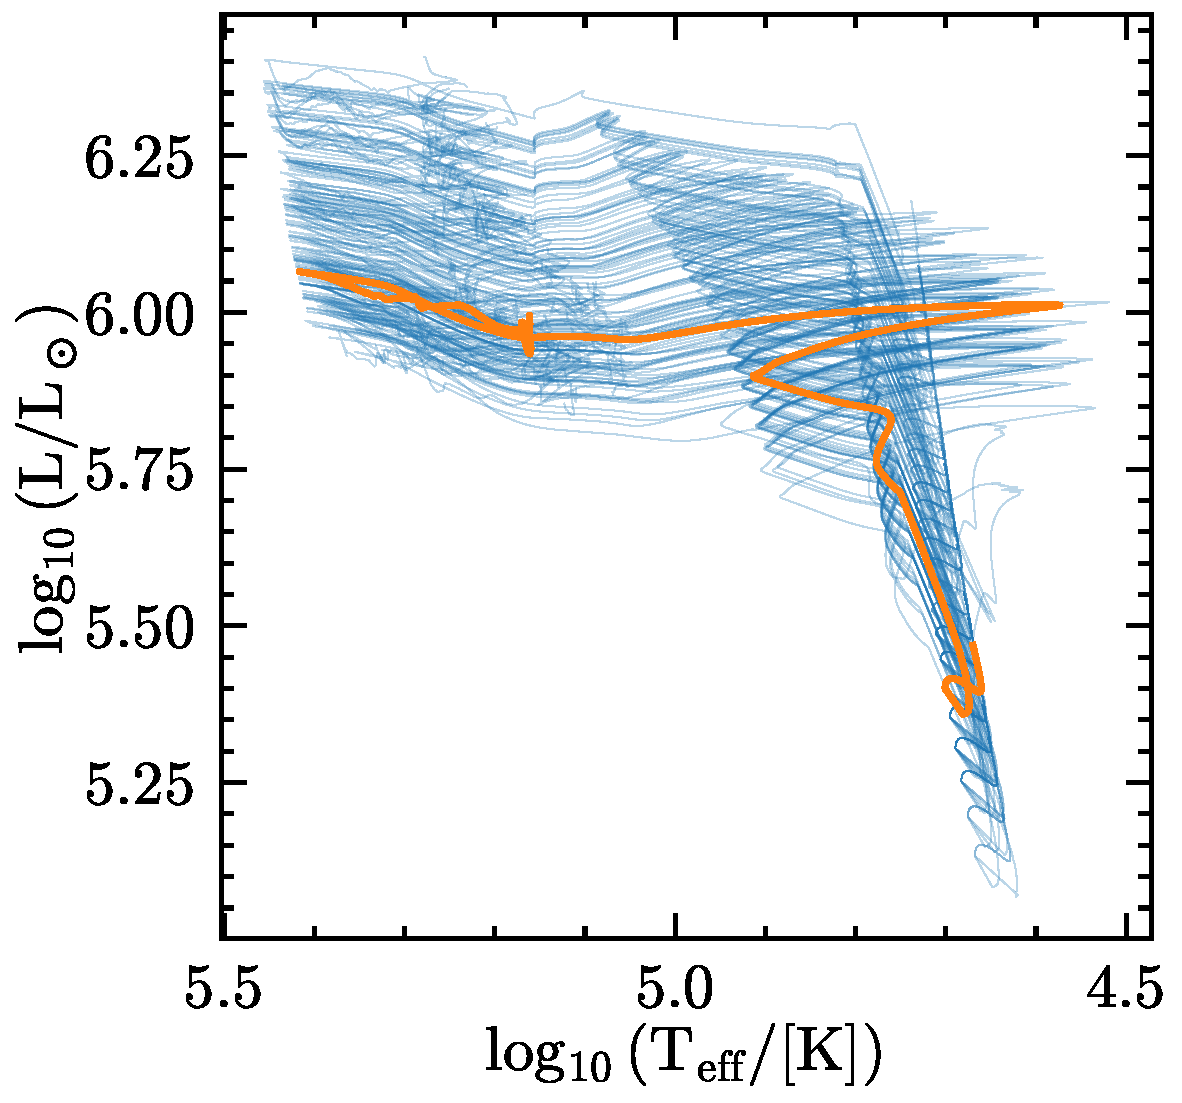
\includegraphics[width=0.5\textwidth]{HRD_grid}
%   \caption{Herzsprung-Russel diagram of rotationally-induced CHE
%     single star models. The orange thick line marks a representative
%     $40M_{\odot}$, $\omega=0.6\omega_{\rm crit}$ model to guide the
%     eye.}
%   \label{fig:HRD}
% \end{figure}



% \begin{figure}[htbp]
%   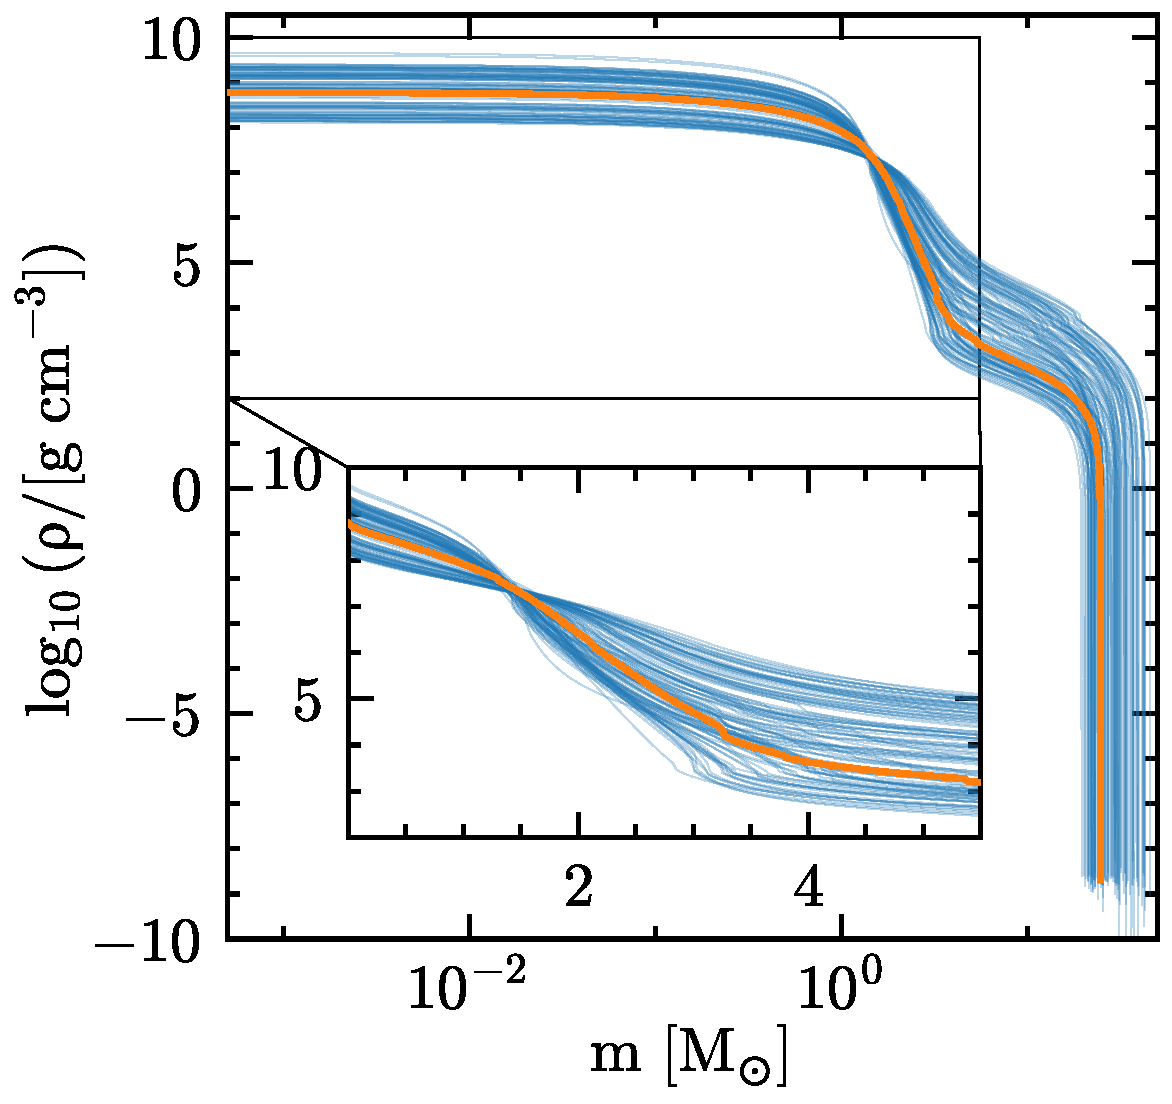
\includegraphics[width=0.5\textwidth]{rho_grid}
%   \caption{Density profiles as a function of Lagrangian mass
%     coordinate for rotationally-induced CHE
%     single star models. The orange thick line marks a representative
%     $40M_{\odot}$, $\omega=0.6\omega_{\rm crit}$ model to guide the
%     eye. The inset focuses on the innermost $m\le5\,M_{\odot}$.}
%   \label{fig:rho}
% \end{figure}



% \begin{figure}[htbp]
%   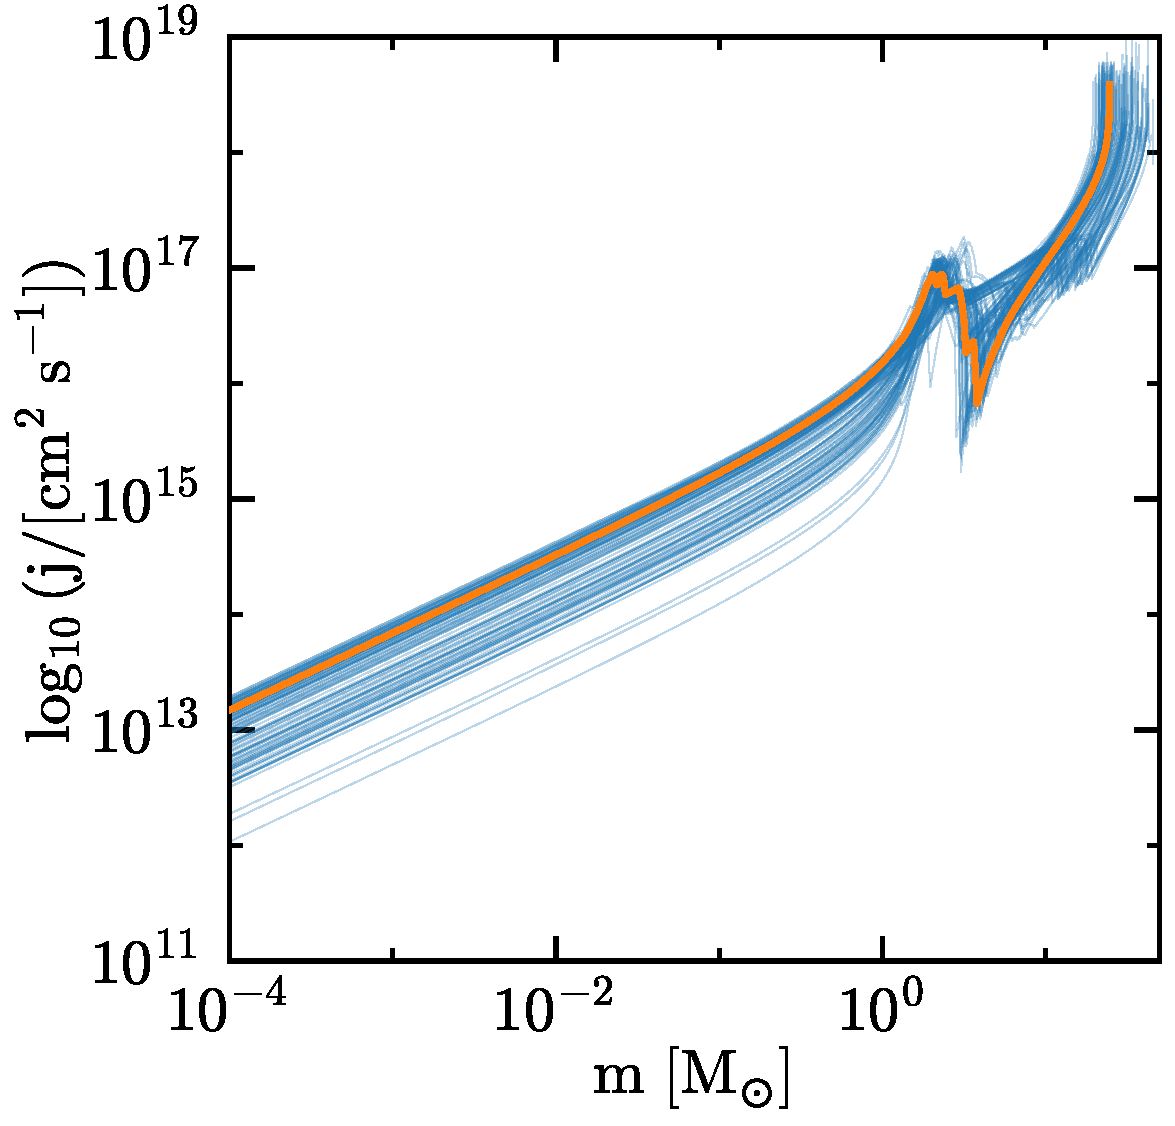
\includegraphics[width=0.5\textwidth]{j_grid}
%   \caption{Specific angular momentum $j=r\omega^{2}$ profiles as a
%     function of Lagrangian mass coordinate for rotationally-induced
%     CHE single star models. The orange thick line marks a
%     representative $40M_{\odot}$, $\omega=0.6\omega_{\rm crit}$ model
%     to guide the eye.}
%   \label{fig:rho}
% \end{figure}


\end{document}

%%% Local Variables:
%%% mode: LaTeX
%%% TeX-master: t
%%% End:
